% concatenated from Isoperimetric.tex
\documentclass[leqno]{article}
\usepackage{amsmath}
\usepackage{amsthm}
\usepackage{amssymb}
\usepackage{graphicx} % Required for inserting images
\usepackage{xcolor}
\usepackage{tikz}
\usepackage{url}
\usepackage{hyperref}
\usepackage{caption}
\usetikzlibrary{angles, quotes, intersections, calc}
\usepackage{pgfplots}
\pgfplotsset{compat=1.18}

\captionsetup[figure]{hypcap=false}

\numberwithin{equation}{section} 
\newtheorem{theorem}[equation]{Theorem}
%\newtheoremj{theorem}{Theorem}[section]
\theoremstyle{definition}
\newtheorem{definition}[equation]{Definition}
%\newtheorem{definition}[theorem]{Definition}
\theoremstyle{remark}
\newtheorem{note}[equation]{Remark}
%\newtheorem{note}[theorem]{Note}
\theoremstyle{plain}
\newtheorem{lemma}[equation]{Lemma}
%\newtheorem{lem}[theorem]{Lemma}
\newtheorem{corollary}[equation]{Corollary}
%\newtheorem{corollary}[theorem]{Corollary}
%\newtheorem{example}{Example}[section]
\newtheorem{proposition}[equation]{Proposition}
\newcommand{\ds}{\displaystyle}
\newcommand{\defeq}{\stackrel{\text{def}}{=}}

\title{Remarks on the relative isoperimetric profile of polygonal domains in $\mathbb{R}^2$}
\author{Jason DeVito, Robert DeYeso III,\\ Ezra Nance, Robert Niedzialomski}
\date{}




\begin{document}

\maketitle

\begin{abstract}
We develop techniques for solving the relative isoperimetric problem on polygonal domains in $\mathbb{R}^2$, with special attention paid to corners.  As an application, we solve the relative isoperimetric problem for a square with a square corner removed.
\end{abstract}


\section{Introduction}



Let $Q\subseteq \mathbb{R}^n$ be a measurable subset with non-zero measure $|Q|$. For any measurable subset $S\subseteq Q$, we let $P(S)$ denote the \textit{relative perimeter} of $S$, that is, the perimeter of $S$ in the interior of $Q$.  For each positive number $t\leq |Q|$, we define $f_{Q}(t) := \inf \{P(S): S\subseteq Q \text{ and } |S| = t\}$.  The function $f_Q$ is called the \textit{relative isoperimetric profile} of $Q$, and any subset $S$ which achieves this infimum is called an \textit{isoperimetric minimizer}.

Several necessary conditions are known about these minimizing subsets. For instance, any minimizer which intersects the boundary of $Q$ must do so orthogonally. However, orthogonality loses all meaning if $\partial Q$ is not smooth at the intersection point. Since these non-smooth points cause complications, often smoothness conditions are assumed on the boundary of $Q$, see for example \cite{CGR,MBNPR,SZ}. %But of course, we would like to remove this assumption.

Our primary goal in this article is to work towards removing the smoothness assumption on $\partial Q$. Specifically, we focus on the case when $Q$ is a polygonal domain, that is, a subset of $\mathbb{R}^2$ bounded by a piecewise linear curve. In Section~ \ref{sec:tools} we characterize all possible ways that an isoperimetric minimizer can interact with corners of a polygonal domain. Our main result is the following.

\begin{theorem}\label{thm:main2}
Let $Q\subseteq \mathbb{R}^2$ be a polygonal region and let $K\in Q$ be a corner. Suppose $S$ is an isoperimetric minimizer. \begin{enumerate}\item If $K$ is convex, then $\partial S$ does not contain $K$.

\item  If $K$ is non-convex, then at most one smooth boundary component of $\partial S$ contains $K$, and this smooth boundary component does not make an acute angle with either of the two edges of $Q$ which contain $K$.
\end{enumerate}
\end{theorem}

The rest of this article is dedicated to the study of a specific family of polygonal domains. We consider the 1-parameter family of the unit square with a square corner removed, that is, $Q_a := [0,1]^2 \setminus [0,a)^2$. These regions were chosen because they offer a relatively simple example of a polygonal domain with a non-convex corner. Furthermore, when $a=0$ we obtain the full unit square, which has already been analyzed in \cite{BB}. This article generalizes their result.
 
Let $f_a$ be shorthand for $f_{Q_a}$. In \cite{BB}, descriptions of isoperimetric minimizing regions were provided as well as an explicit formula for $f_0$. We do the same for $f_a$ for all $a \in [0,1)$. Our main result is the following.

\begin{theorem}\label{thm:main}For each $a\in [0,1)$ and $t\leq|Q_a|$, isoperimetric minimizers are given by one of the regions $S_1,S_2,S_3$ or $S_4$ in Figure \ref{fig:main}.  An explicit formula for $f_a$ is given by equation \eqref{eq:profile}.
\end{theorem}

It is interesting that $f_a$ goes through phase changes as $a$ increases. For small $a$, only $S_1$ and $S_2$ regions arise, that is, $f_a$ agrees with the formula found in \cite{BB}. However, once $a$ becomes larger, we must also consider $S_4$ regions, which can intersect the non-convex corner at unusual angles.  For even larger values of $a$, $S_3$ regions become relevant.

It follows from our proof that every isoperimetric minimizer must be a region of the form $S_1,S_2,S_3$, or $S_4$.  In addition, for each $a$ and all but finitely many $t$, it follows from our proof that a minimizing region $S$ is unique up to the obvious symmetries, e.g, a quarter circle can be placed in any of the five convex corners. 

As an important corollary, this example shows that the boundary of a minimizer can intersect a non-convex corner, so that Theorem~\ref{thm:main2}(2) is sharp.

\begin{center}
    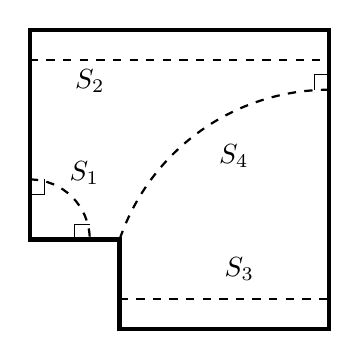
\begin{tikzpicture}[scale=3.8]
        \draw[ultra thick] (0.3,0) -- (1,0) -- (1,1) -- (0,1) -- (0,0.3) -- (0.3,0.3) -- cycle;
        \draw[thick, dashed] (0,.9) -- (1,.9);
        \draw[thick, dashed] (.3,0.1) -- (1,0.1);
        \draw[thick, dashed] (1.0,0.8) arc (90:161:0.74);
        \draw (0,0.45) -- (.05,0.45) -- (0.05, .5);
        \draw (.15,.3) -- (.15,.35) -- (.2,.35);
        \draw[thick, dashed] (0,.5) arc (90:0:.2);
        \draw (1,0.85) -- (0.95,0.85) -- (0.95,0.8);
        %\draw (0.29,0.15) node[anchor=east] {$a$};
        %\draw (0.65,0) node[anchor=north] {$1-a$};
        \draw (0.60,0.65) node[anchor=north west] {$S_4$};
        \draw (.1,.45) node[anchor = south west] {$S_1$};
        \draw (.2, .9) node[anchor = north] {$S_2$};
        \draw (.7, .13) node [anchor = south] {$S_3$};
    \end{tikzpicture}
    \captionof{figure}{Region $S_1$ is a quarter circle hitting both boundary components of $Q_a$ perpendicularly.  Regions $S_2$ and $S_3$ are bounded by line segments parallel to the sides of $Q_a$, and the boundary of Region $S_4$ is a portion of a circle connecting the non-convex corner to a side of length 1.}\label{fig:main}
\end{center}

\textbf{Acknowledgements}  The first author was supported by the NSF through DMS-2405266.  He is grateful for the support.



\section{Background}\label{sec:background}

Suppose $Q \subseteq \mathbb{R}^2$ is a polygonal region, i.e., a domain whose boundary is piecewise linear. Let $S\subseteq Q$ be a measurable region with area $|S|$. We denote by $P(S)$ the relative perimeter of $S$ in $Q$.  That is, $P(S)$ is defined by
\begin{equation*}
P(S)=\sup\left\{\int_S\textrm{div} (X)\,dx\colon X\in C^\infty_c(\text{int}(Q),\mathbb{R}^2),\,\|X\|\leq 1\right\},    
\end{equation*}
where $\text{int}(Q)$ is the interior of $Q$ and $\textrm{div} (X)$ is the divergence of the vector field~$X$.

We are interested in determining the \textit{relative isoperimetric minimizers} (or, more briefly, a \textit{minimizer}).  Recall that a minimizer is a measurable subset $S\subseteq Q$ for which  
\[
    P(S)\leq P(S') \text{ for all } S'\subseteq Q \text{ with } |S| = |S'|.  
\]
If $S$ is a minimizer, then its complement $Q \setminus S$ is also a minimizer bounding area $|Q| - |S|$.  In particular, we can always assume that $|S| \leq \frac{1}{2}|Q|$.

We have the following structure result for isoperimetric minimizers adapted to our situation.  The first bullet point  was proven by Gonzalez, Massari, and Tamanini \cite[Theorem 2, pg. 29]{GMT}, while the second two were proven by Grüter \cite[Theorem (iii) pg. 264]{Gr}.

\begin{theorem}
    \label{thm:structure}  
    Let $S\subseteq Q$ be an isoperimetric minimizer.  Then 
    \begin{itemize}
        \item $\partial S\cap \text{int}(Q)$ is an embedded analytic submanifold of $\text{int}(Q)$,
        \item  there is a number $c$ for which $\partial S\cap \text{int}(Q)$ is a disjoint union of curves, all of which have constant mean curvature $c$,
        \item  $\partial S$ intersects the non-corner points of $Q$ orthogonally.
    \end{itemize}
\end{theorem}

It is a priori possible that distinct connected components of $\partial S\cap \text{int}(Q)$ belong to the same connected component of $\partial S$, see Figure \ref{fig:TwoArcsFromCorner}. We define the number of \textit{smooth boundary curves of $S$} as the number of components of $\partial S\cap \text{int}(Q)$.  If no such curves touch an edge or corner of $Q$, this is simply the number of components of $\partial S$ as a topological manifold. In general, $S$ could have multiple smooth boundary components. 

\begin{center}
    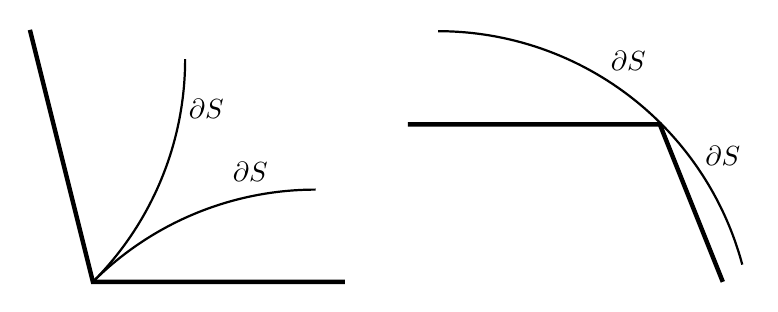
\begin{tikzpicture}[scale=0.8]
        \draw[ultra thick] (4,0) -- (0,0) -- (-1,4);
        \draw[thick] (0,0) arc (-45:0:5);
        \draw[thick] (0,0) arc (135:90:5);
        \node at (2.5,1.75) {$\partial S$};
        \node at (1.8,2.75) {$\partial S$};
    \begin{scope}[shift={(5,0)}]
        \draw[ultra thick] (0,2.5) -- (4,2.5) -- (5,0);
        \draw[thick] (4.015,2.515) arc (45:90:5);
        \draw[thick] (4.015,2.515) arc (45:15:5);
        \node at (3.5, 3.5) {$\partial S$};
        \node at (5, 2) {$\partial S$};
    \end{scope}
    \end{tikzpicture}
    \captionof{figure}{Two examples showing that the boundary of $S$ is a connected topological manifold while $\partial S \cap \text{int}(Q)$ has two smooth components.}\label{fig:TwoArcsFromCorner}
\end{center}

We conclude this section with a proof that for a polygonal region $Q$ and for a minimizer $S$, the boundary $\partial S$ can have at most finitely many smooth connected components.


\begin{proposition}
\label{prop:finiteboundary}
Suppose $Q\subseteq\mathbb{R}^2$ is a polygonal region and $S \subseteq Q$ is relative isoperimetric minimizer.  Then $\partial S$ has finitely many smooth boundary components.
\end{proposition}

\begin{proof}

Suppose for a contradiction that $S$ is a minimizer for which $\partial S$ has infinitely many smooth boundary components.  From Theorem \ref{thm:structure}, the boundary components are either all line segments or all arcs of circles of some fixed radius~$r$.

Suppose initially that the boundary $\partial S$ consists of line segments.  We first claim that there are only finitely many smooth boundary components of $\partial S$ which intersect $Q$ in a corner.  This follows because such a line segment must either intersect one of the finitely many remaining corners or intersect $\partial Q$ perpendicularly, which determines the slope of the segment up to finitely many possibilities.  Since there are infinitely many smooth boundary components, there must be infinitely many which intersect two walls of $Q$ perpendicularly.  But there is a positive minimum such distance between parallel walls of $Q$, while there are infinitely smooth boundary components.  Thus, we find $P(S) = \infty$, a contradiction. 


We next consider the case where there are infinitely many smooth boundary components of $\partial S$ all given by arcs of a circle of radius $r$.  For any two parallel walls of $Q$ there are no such arcs intersecting them orthogonally.  For any two non-parallel walls, in order for a component of $\partial S$ to intersect them both orthogonally, the center of this arc must lie on the lines formed by extending both walls.  Since the radius and center are determined, there is at most one such arc lying in $Q$.  Thus, by hypothesis, there must be infinitely many smooth components intersecting one corner $K$ of $Q$.  For each arc containing $K$, it either ends on a wall of $Q$ or another corner of $Q$.  But for each wall, there are at most two such arcs, because the center of the arc must lie in the line made by extending the wall and the distance to $K$ must be $r$.  And for each corner distinct from $K$ there are at most two arcs containing $K$ and this corner, because the center must simultaneously lie on a circle of radius $r$ about each corner points.  Thus, there are only finitely many arcs of circles of radius $r$ satisfying the condition that they meet walls of $Q$ orthogonally, contradicting the fact that there are infinitely many smooth components.

\bigskip




%Due to Theorem \ref{thm:structure}, $\partial S$ consists either of line segments or of circular arcs each with the same radius $r_S$. Since $\partial S$ is analytic within $\text{int}(Q)$, its components accumulate toward a point $z \in Q$. Since $S$ is compact in $Q$, we further have that $z \in S$. 

%Let $U \subseteq Q$ be a neighborhood containing $z$. If $\partial S$ contains infinitely-many straight line segments $\{L_i\}$ accumulating toward $z$, then
%\[
%    P(S) \geq P(S \cap U) \geq \sum_i^{\infty} P(L_i \cap U)
%\]
%diverges since $P(L_i \cap U) \not\rightarrow 0$. This contradicts $S$ being a minimizer, and so $\partial S$ must contain finitely-many straight line segments. We cannot have a sequence of circles accumulate toward $z$ since this would contradict each having the same radius. Together, these statements obstruct $z \in \text{int}(Q)$ as only a sequence of lines or a sequence of circles could realize its accumulation. Then we must have $z \in \partial Q$, and that a sequence of circular arcs accumulates toward $z$.

%We know that $z$ cannot be a corner of $Q$ due to Theorem \ref{thm:corner}\footnote{{\color{blue} The proof of Theorem 3.1 uses finiteness of $\partial S$, so this is circular}}, and so $z$ must lie on an edge $E_z$ of $Q$. Any circular arc that accumulates toward $z$ must intersect $E_z$ orthogonally, and intersect either another edge $E'$ orthogonally or some corner of $Q$. However, a circle that intersects $E_z$ and $E'$ orthogonally necessarily has center $\widetilde{E}_z \cap \widetilde{E'}$, where $\widetilde{E}$ represents the (infinite) line containing $E$ in $\mathbb{R}^2$. This shows that any pair of edges of $Q$ admits at most one circular arc of $\partial S$, and a similar argument shows this holds for any pair of edge and corner of $Q$. Then $\partial S$ containing infinitely-many circular arcs contradicts $Q$ having finitely-many edges and corners. This exhausts all potential ways of $\partial S$ having infinitely-many components, and completes the proof. \\
\end{proof}




\section{An analysis of corners}\label{sec:tools}  In this section, we carry out a detailed analysis of how the boundary curves of an isoperimetric minimizer can intersect corners of a polygonal region $Q\subseteq \mathbb{R}^2$.  In particular, we show that $\partial S$ cannot intersect a convex corner and that at most one smooth component of $\partial S$ can intersect each non-convex corner.  %Later, we will have a general result which guarantees that an isoperimetric profile function for connected regions is automatically the isoperimetric profile for all regions.

\begin{theorem}\label{thm:corner}
Let $Q\subseteq \mathbb{R}^2$ be a polygonal region and let $K\in Q$ be a corner. Suppose $S$ is an isoperimetric minimizer. \begin{enumerate}\item If $K$ is convex, then $\partial S$ does not contain $K$.

\item  If $K$ is non-convex, then at most one smooth boundary component of $\partial S$ contains $K$, and this smooth boundary component does not make an acute angle with either of the two edges of $Q$ which contain $K$.
\end{enumerate}
\end{theorem}

When we compute the relative isoperimetric profile of the region $Q_a$, we will see that in some situations the boundary of an isoperimetric minimizer must intersect the non-convex corner of $Q_a$.  In particular, Theorem~\ref{thm:corner}(2) is sharp.  We will prove the theorem after establishing a number of preliminary propositions.  

\begin{proposition}\label{prop:circleTangentToSide} Let $Q\subseteq\mathbb{R}^2$ be a polygonal region and let $K\in Q$ be a convex corner.  Suppose that $S\subseteq Q$ has a unique smooth component containing $K$.  If this component is tangent to $Q$ at $K$, then $S$ is not an isoperimetric minimizer.
\end{proposition}

\begin{proof} By way of contradiction, assume that $S$ is an isoperimetric minimizer. We will find a new region $S'$ with $|S'| = |S|$ and with $P(S') < P(S)$.

Since $\partial S$ has constant mean curvature, the fact that it is tangent to $Q$ at $K$ implies that the smooth component of $\partial S$ containing $K$ is an arc of a circle.   Let $Q_1$ denote the side of $Q$ which is tangent to the arc.

\begin{center}
    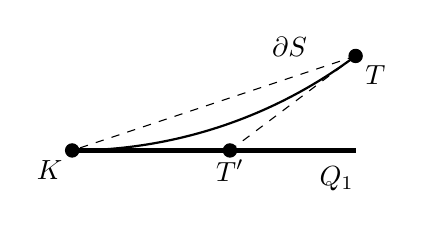
\begin{tikzpicture}[scale=1.2]
        \draw[ultra thick] (0,-5) -- (3,-5);
        \filldraw (0,-5) circle (2pt) node[anchor=north east] {$K$};
        \draw (2.3,-3.9) node {$\partial S$};
        \draw (2.8,-5.3) node {$Q_1$};
        \draw[thick] (0,-5) arc (-90:-53.13:5);
        \draw[dashed] (3,-4) -- (0,-5);
        \draw[dashed] (3,-4) -- (1.67,-5) node[anchor=north] {$T'$};
        \filldraw (1.67,-5) circle (2pt);
        \filldraw (3,-4) circle (2pt) node[anchor=north west] {$T$};
    \end{tikzpicture}
    \captionof{figure}{Neighborhood of a corner $K$ with a circular arc.}\label{fig:arcTangentToCorner}
\end{center}

By Proposition \ref{prop:finiteboundary}, $\partial S$ has only finitely many smooth boundary components. Therefore, we may find a neighborhood of $K$, which intersects $\partial S$ only in a portion of this circular arc.  Given any point $T$ on this circular arc, we let $T'$ denote the intersection of the tangent line at $T$ and $Q_1$, see Figure \ref{fig:arcTangentToCorner}.  By choosing $T$ close enough to $K$ on the circular arc, we may assume that the angle $\angle TKT'$ is acute and the angle $
\angle TT'K$ is obtuse.

The secant line from $T$ to $K$ is shorter than the circular arc between these points.  Moreover, since the angle $\angle KT'T$ is obtuse, it follows that as we deform the secant line to the tangent line through a family of line segments, the lengths decrease.  In particular, they are all shorter than the circular arc.

By replacing $S$ with its complement, we assume without loss of generality that the region $S$ lies inside the circular arc.   It then follows that the secant line underestimates the area while the tangent line overestimates it.  In particular, by continuity, there is some line segment in the deformation whose area agrees with the area of $S$.  Thus, by replacing the arc by this line segment, we obtain the desired subset~$S'$.

\end{proof}


The following lemma will allow us to extend results concerning line segments to circular arcs.  Proposition \ref{prop:convexcorner} contains the key construction in proving Theorem \ref{thm:corner}.


\begin{lemma}\label{lem:chordAreaOrder}Suppose $C$ is a circle of radius $r$.  Then the smaller area determined by a chord of length $\ell$ has area  $O(\ell^3)$.
\end{lemma}

\begin{proof}
The area is given by $g(\ell):=\frac{1}{2} r^2 \left(2\arcsin\left(\frac{\ell}{2r}\right)-\sin\left(2\arcsin\left(\frac{\ell}{2r}\right)\right)\right)$.
 An easy calculation shows that $g(0)=\frac{dg}{d\ell}(0) = \frac{d^2 g}{d\ell^2}(0)= 0$, but $\frac{d^3g}{d\ell^3}(0) = \frac{1}{2r}\neq 0$.
\end{proof}







\begin{proposition}\label{prop:convexcorner}Suppose $Q\subseteq\mathbb{R}^2$ is a polygonal region and $K\in Q$ is a convex corner.  Suppose $S\subseteq Q$ and $\partial S$ contains exactly one smooth component containing $K$, which is either a line segment or an arc of a circle.  Then there exists $S' \subseteq Q$, an arbitrarily small deformation of $S$, with the following properties:

\begin{itemize}\item $|S| = |S'|$
\item $P(S) > P(S')$
\item No smooth component of $\partial S'$ contains $K$.
\end{itemize}

\end{proposition}

\begin{proof}
    We will first consider the case when the smooth boundary component containing $K$ is a line segment. For a small enough neighborhood of $K$, we can consider only the corner and this single line segment. Let $P$ be a point on $\partial S$ and let $\ell$ be the length of this line. Note that since $K$ is a convex corner, $\partial S$ makes at least one acute angle with $\partial Q$. Thus, without loss of generality, we have the following picture for a neighborhood of $K$.

    \begin{center}
        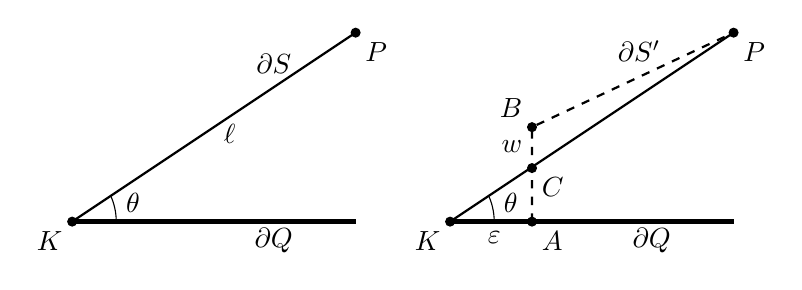
\begin{tikzpicture}[scale=0.8]
            \draw[ultra thick] (-4.5,2) -- (0,2);
            \draw[thick] (-4.5,2) -- (0,5);
            \filldraw (-4.5,2) circle (2pt) node[anchor=north east] {$K$};
            \draw (-2,3.4) node {$\ell$};
            \draw (-1.3,4.5) node {$\partial S$};
            \draw (-1.3,1.7) node {$\partial Q$};
            %\draw[thick] (-4.5,2) arc (156.4:91:5);
            \draw (-3.8,2) arc (0:25:1);
            \draw (-3.8,2.3) node[anchor=west] {$\theta$};
            \filldraw (0,5) circle (2pt) node[anchor=north west] {$P$};
            \begin{scope}[shift={(6,0)}]
                \draw[ultra thick] (-4.5,2) -- (0,2);
                \draw[thick] (-4.5,2) -- (0,5);
                \filldraw (-4.5,2) circle (2pt) node[anchor=north east] {$K$};
                \filldraw (-3.2,2) circle (2pt) node[anchor=north west] {$A$};
                \filldraw (-3.2,3.5) circle (2pt) node[anchor=south east] {$B$};
                \draw (-3.8,2) node[anchor=north] {$\varepsilon$};
                %\draw (-2,3.4) node {$\ell$};
                \draw (-3.2,3.2) node[anchor=east] {$w$};
                \draw (-1.5,4.7) node {$\partial S'$};
                \draw (-1.3,1.7) node {$\partial Q$};
                \draw (-3.8,2) arc (0:25:1);
                \draw (-3.8,2.3) node[anchor=west] {$\theta$};
                \filldraw (0,5) circle (2pt) node[anchor=north west] {$P$};
                \draw[thick,dashed] (-3.2,2) -- (-3.2, 3.5) -- (0,5);
                \filldraw (-3.2,2.85) circle (2pt) node[anchor=north west] {$C$};
            \end{scope}
        \end{tikzpicture}
        \captionof{figure}{On the left we have $\partial S$ intersecting a corner $K$. On the right we have a deformation $\partial S'$ which avoids corner $K$.}\label{fig:deformAwayFromCorner}
    \end{center}

    We will now deform $\partial S$ to $\partial S'$ with the desired properties. Consider a point $A$ which is $\varepsilon$ units away from the corner, and let $B$ be the point directly above $A$ so that $|S| = |S'|$. Let $C$ be the intersection point of $\overline{KP}$ and $\overline{AB}$, and let $w$ be the length of $\overline{BC}$. Note that in order for $|S| = |S'|$, we need the triangles $\Delta ACK$ and $\Delta BCP$ to have the same area. In other words, we need $$\frac{1}{2}\varepsilon^2 \tan\theta = \frac{1}{2}(\ell - \varepsilon\sec\theta)w\cos\theta.$$ This is true when
    \[
        w = \frac{\varepsilon^2\tan\theta}{\ell\cos\theta - \varepsilon}.
    \]
    Having achieved that $|S| = |S'|$, we now compare perimeters of the boundaries.  Note that $P(S) > P(S')$ if and only if $\left|\,\overline{KP}\,\right| > \left|\,\overline{AB}\,\right| + \left|\,\overline{BP}\,\right|.$
    As $|\overline{KP}|  = |\overline{KC}| + |\overline{CP}|$, it follows from the triangle inequality that this inequality is true if
    \begin{equation}\label{eq:lowerPerim}
        \left|\,\overline{KC}\,\right| > 
        2\left|\,\overline{BC}\,\right| + 
        \left|\,\overline{AC}\,\right|.
    \end{equation}
    Indeed, \begin{align*} |\overline{KP}| &= |\overline{KC}|+|\overline{PC}|\\
    & > 2|\overline{BC}| +|\overline{AC}| + |\overline{PC}|\\
    &= (|\overline{BC}| + |\overline{AC}|) + (|\overline{BC}| + |\overline{PC}|)\\
    & \geq |\overline{AB}| + |\overline{BP}|.\end{align*}
    
    Substituting into inequality \eqref{eq:lowerPerim} and rearranging, we find that inequality \eqref{eq:lowerPerim} holds if and only if 
    \begin{equation}\label{eq:lowerPerim2}
        2\varepsilon^2\tan\theta < \varepsilon(\ell - \varepsilon\sec\theta)(1-\sin\theta).
    \end{equation}
    Notice that since $\theta \in (0,\tfrac{\pi}{2})$, all factors in (\ref{eq:lowerPerim2}) are positive.  In addition, the left side is $O(\varepsilon^2)$ while the right side is $O(\varepsilon)$.  It follows that for all sufficiently small $\varepsilon$, the inequality \eqref{eq:lowerPerim2} holds. Hence, the proof is complete in the case where the smooth boundary component of $\partial S$ is a line segment.

    Now we will consider the case when the smooth boundary component containing $K$ is the an of a circle. By Proposition \ref{prop:circleTangentToSide}, we can assume that $\partial S$ does not touch $K$ tangentially to $Q$. Furthermore, since $K$ is a convex corner, $\partial S$ makes an acute angle at $K$ with at least one side of $\partial Q$. Thus, without loss of generality, we can assume that we have a neighborhood of $K$ which looks like one of the following, depending on the curvature.

    \begin{center}
        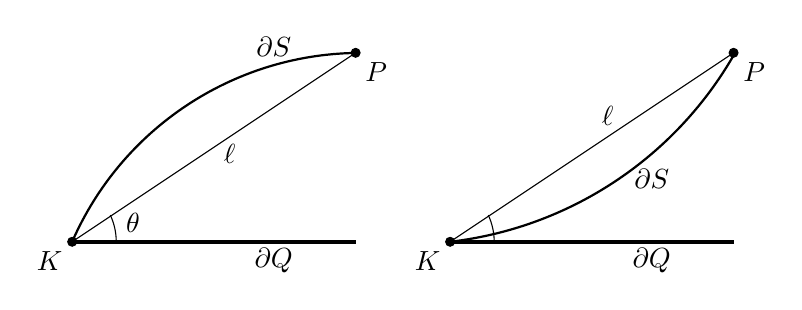
\begin{tikzpicture}[scale=0.8]
            \draw[ultra thick] (-4.5,2) -- (0,2);
            \draw (-4.5,2) -- (0,5);
            \filldraw (-4.5,2) circle (2pt) node[anchor=north east] {$K$};
            \draw (-2,3.4) node {$\ell$};
            \draw (-1.3,5.1) node {$\partial S$};
            \draw (-1.3,1.7) node {$\partial Q$};
            \draw[thick] (-4.5,2) arc (156.4:91:5);
            \draw (-3.8,2) arc (0:25:1);
            \draw (-3.8,2.3) node[anchor=west] {$\theta$};
            \filldraw (0,5) circle (2pt) node[anchor=north west] {$P$};
        \begin{scope}[shift={(6,0)}]
            \draw[ultra thick] (-4.5,2) -- (0,2);
            \draw (-4.5,2) -- (0,5);
            \filldraw (-4.5,2) circle (2pt) node[anchor=north east] {$K$};
            \draw (-2,4) node {$\ell$};
            \draw (-1.3,3) node {$\partial S$};
            \draw (-1.3,1.7) node {$\partial Q$};
            \draw[thick] (-4.5,2) arc (-83.34:-30:6);
            \draw (-3.8,2) arc (0:25:1);
            \filldraw (0,5) circle (2pt) node[anchor=north west] {$P$};
        \end{scope}
        \end{tikzpicture}
        \captionof{figure}{Both possibilities for a circular arc to touch a corner acutely.}\label{fig:arcTouchingCorner}
    \end{center}
    
    Consider a point $P \in \partial S$, and let $\ell$ be the length of the secant line $\overline{KP}$. Now we can repeat the argument for the straight line case to create $\partial S'$ away from corner $K$. The only difference is that now $w$ will have to take into account the area, say $\delta$, between $\partial S$ and the secant line $\overline{KP}$. By doing this we can ensure that $|S| = |S'|$. Following the same logic as before, we will have that $P(S) > P(S')$ if
    \begin{equation}\label{eq:lowerPerim3}
        2\varepsilon^2\tan\theta  \pm \delta < \varepsilon(\ell - \varepsilon\sec\theta)(1-\sin\theta).
    \end{equation}
    Let $\varepsilon = \lambda \ell$. By Lemma \ref{lem:chordAreaOrder}, $\delta = O(\ell^3)$. Therefore, inequality \eqref{eq:lowerPerim3} is true if and only if there exists some $\lambda \in (0,1)$ and some $\ell > 0$ such that
    \[
        2\lambda^2\ell^2\tan\theta  \pm O(\ell^3) < \lambda\ell^2(1 - \lambda\sec\theta)(1-\sin\theta).
    \]
    We divide by $\ell^2$ and rearrange to see that inequality \eqref{eq:lowerPerim3} is true if and only if
    \[
        O(\ell) < \lambda(1-\sin\theta) - \lambda^2\sec\theta(1+\sin\theta).
    \]
    Let $\theta_{1}$ be the larger of the two angles formed by the tangent line at $K$ and the secant line at $K$. Then
    \[
        \lambda(1-\sin\theta_{1}) - \lambda^2\sec\theta_{1}(1+\sin\theta_{1}) < \lambda(1-\sin\theta) - \lambda^2\sec\theta(1+\sin\theta)
    \]
 for any $0\leq \theta < \theta_1$.   Thus, we have $P(S) > P(S')$ if
    \[
        O(\ell) < \lambda(1-\sin\theta_{1}) - \lambda^2\sec\theta_{1}(1+\sin\theta_{1}).
    \]
    We can choose $\lambda \in (0,1)$ so that the right-hand side is positive. Also, since the right-hand side is independent of $\ell$, we can then shrink $\ell$ to achieve our result. The circular arc case is done.
\end{proof}

%Notice that the same argument would also work if we considered a single smooth component touching a wall of $\partial Q$. This shows that if $S \subseteq Q$ is a minimizer, then $\partial S$ can only touch walls orthogonally. This, of course, is a result in the classical isoperimetric theory that we have recovered. 

Now we will move to the case when more than one smooth boundary component is touching a corner.

\begin{proposition}\label{prop:anycorner}Suppose $Q\subseteq\mathbb{R}^2$ is a polygonal region and $K\in Q$ is a corner.  Suppose $S\subseteq Q$ and $\partial S$ contains exactly two smooth components containing $K$ and that the interior angle of these two smooth components does not contain the corner sides at $K$.  Then there exists $S' \subseteq Q$, an arbitrarily small deformation of $S$, with the following properties:

\begin{itemize}\item $|S| = |S'|$
\item $P(S) > P(S')$
\item No smooth component of $\partial S'$ contains $K$.
\end{itemize}

\end{proposition}

\begin{proof}
    Since the interior angle these components make does not contain the corner sides, the angle within $Q$ is less than $\pi$. Hence, that angle bisected will be acute. Also, from Theorem \ref{thm:structure}, we have that these two smooth components of $\partial S$ which contain $K$ have the same curvature. Thus, we can simply bisect the interior angle and run the argument from Proposition \ref{prop:convexcorner} on each side to create an arbitrarily small deformation of $S$ with the desired properties. 
\end{proof}

We are ready to prove Theorem \ref{thm:corner}.

\begin{proof}[Proof of Theorem \ref{thm:corner}]  Let $K$ be a corner and let $Q_1$ and $Q_2$ denote the two sides of $Q$ containing $K$.  For both statements $(1)$ and $(2)$, we will prove the contrapositive.

$(1)$ Assume that $K$ is a convex corner.  Our goal is to show that if $\partial S$ contains at least one smooth boundary components containing $K$, then $S$ is not an isoperimetric minimizer.  If there is exactly one smooth component of $\partial S$ containing $K$, it makes an acute angle with at least one of $Q_1$ or $Q_2$.  Then the result follows from either Proposition \ref{prop:convexcorner} or Proposition \ref{prop:circleTangentToSide}, depending on the measure of this angle.

Thus, we assume there are at least two smooth boundary components of $\partial S$ containing $K$.  If we fix a side, say $Q_1$, of $Q$ containing $K$, then we observe that the angles at $K$ between $Q_1$ and each smooth component of $\partial S$ are almost distinct: if the smooth boundary components are segments, they must be distinct while if they are arcs of circles, at most two share an angle, see Figure \ref{fig:tangent}.  This follows because each smooth component of $\partial S$ has the same curvature. Hence, if they agree to first order and they have the same concavity relative to $Q_1$, then they are the same smooth boundary component.


\begin{center}
\centering
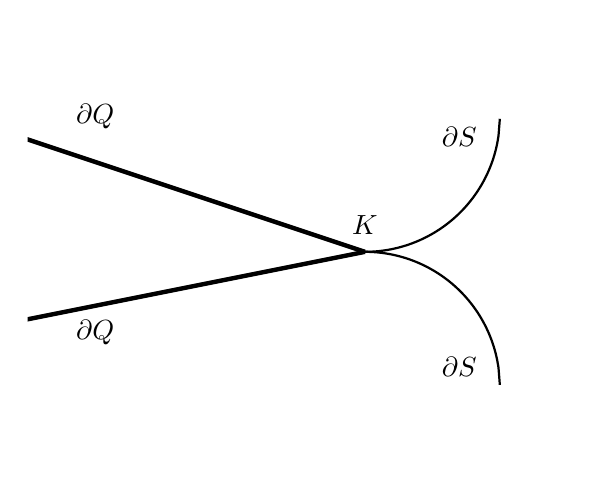
\begin{tikzpicture}
    \begin{axis}[
        axis lines = middle,
        ticks = none,
        xlabel = {},
        ylabel = {},
        xmin = -2.5, xmax = 1.5,
        ymin = -1.5, ymax = 1.5,
        axis line style = {draw=none}, % Remove the axis lines entirely
        axis equal
    ]
        % Graph of f(x) = -1/3 * x for -3 <= x <= 0
        \addplot [
            domain=-3:0, 
            samples=2, 
            ultra thick, 
            black
        ] {-1/3 * x};
        
        % Graph of g(x) = 1/4 * x for -3 <= x <= 0
        \addplot [
            domain=-3:0, 
            samples=2, 
            ultra thick, 
            black
        ] {1/5 * x};
        
        % Graph of h(x) = 1 - sqrt(1 - x^2) for 0 < x <= 1
        \addplot [
            domain=0:1, 
            samples=100, 
            thick, 
            black
        ] {1 - sqrt(1 - x^2)};
        
        % Graph of j(x) = sqrt(1 - x^2) - 1 for 0 < x <= 1
        \addplot [
            domain=0:1, 
            samples=100, 
            thick, 
            black
        ] {sqrt(1 - x^2) - 1};

\draw (-2,1) node {$\partial Q$};
\draw (-2,-0.6) node {$\partial Q$};
\draw (0.7,0.85) node {$\partial S$};
\draw (0.7,-0.85) node {$\partial S$};
\draw (0,0.2) node {$K$};

       
    \end{axis}
\end{tikzpicture}
\captionof{figure}{Two smooth boundary components which are tangent at $K$.}\label{fig:tangent}
\end{center}

Since the angle is convex, any smooth boundary component must make an acute angle with at least one side of $Q$, say $Q_1$, at $K$.  Choose the smooth boundary component making the least angle with this side; if there are two, choose the circular arc which locally bends towards $Q_1$.  Now, we apply the proof of Proposition \ref{prop:convexcorner} or the proof of Proposition \ref{prop:circleTangentToSide} to this smooth boundary component. As long as this new smooth boundary component does not intersect the other smooth boundary components of $\partial S$, we obtain a region $S'$ with the same area but smaller perimeter.  

From the proof of Proposition \ref{prop:convexcorner}, the segment $w=\overline{CB}$ has length $O(\varepsilon^2)$.  Since the separation between different smooth components of $\partial S$ grows as $O(\varepsilon)$ and there are only finitely many smooth components, it follows that for $\varepsilon$ sufficiently small, the new boundary component of $S'$ does not intersect any of the other boundary components of $S$.

In addition, from the proof of Proposition \ref{prop:circleTangentToSide}, if we select $T$ such that the angle $\angle TKT'$ is smaller than the second smallest angle made at $K$, then the secant line between $K$ and $T$ does not intersect any other smooth boundary component of $\partial S$, and thus, none of the interpolating line segments does either. Therefore, in this case, we may form $S'$ in such a way that the new smooth boundary component does not intersect any of the other smooth boundary components of $S$. This completes the proof of $(1)$.

\bigskip

$(2)$  We will prove the contrapositive.  Assume that $\partial S$ contains at least two smooth boundary components containing $K$.  If any such smooth boundary component makes an acute angle with either of the two sides of $Q$ containing $K$, we repeat the proof of $(1)$ to show that $S$ is not an isoperimetric minimizer.  Thus, we may assume that all smooth boundary components make an obtuse or right angle with the two sides of $Q$ containing $K$.  It follows that any two smooth boundary components of $\partial S$ satisfy the hypothesis of Proposition \ref{prop:anycorner}.

As in the proof of (1), the angles made by any smooth boundary component of $\partial S$ and $Q_1$ are almost distinct.  Choose two such smooth boundary components for which the angle between them is minimized.  (If this minimum is achieved by multiple pairs of smooth boundary components, choose any pair of them.)  Now we apply the construction used in the proof of Proposition \ref{prop:anycorner}.  This completes the proof as long as the newly constructed smooth boundary components of $\partial S'$ do not intersect any of the other smooth boundary components of $\partial S$. By minimality of the angle, there are no smooth boundary components of $\partial S$ lying between the two modified smooth boundary components. And, since $w$ is $O(\varepsilon^2)$, we can argue as in the proof of $(1)$ to complete the proof.

\end{proof}













\iffalse

This proposition addresses the case when $\partial S$ touches a corner of $Q$ and forms an acute angle, see Figure \ref{fig:acuteCornerDeform}.

\begin{proposition}\label{prop:acuteCorner}
    Suppose $Q \subseteq \mathbb{R}^2$ is any polygonal region with corner $K\in Q$ and suppose $S \subseteq Q$ is <what hypothesis?> Suppose that $\partial S$ contains exactly one smooth component containing $K$ that this component is a line segment.  Assume additionally that this component forms an acute angle at $K$ with at least one side of $Q$.  Then $S$ is not an isoperimetric minimizer.
\end{proposition}

\begin{proof}

    By way of contradiction, suppose $S$ is an isoperimetric minimizer containing a unique boundary component containing $K$, and that this boundary component is a line segment.  We will show that we can deform $S$ to a new region $S'$ with $|S| = |S'|$ and with $P(S') < P(S)$, contradicting minimality of $S$.

    We will now focus on this corner, as shown in Figure \ref{fig:shortline}.  In this figure, $\overline{KD}$ is a portion of $\partial S$ While $\overline{KA}$ is a portion of $\partial Q$.   Now we will deform $\partial S$, which consists of $\overline{KD}$, to a new boundary $\partial S'$, which consists of $\overline{AB}$, $\overline{BC}$, and $\overline{CD}$.
\begin{figure}
    \begin{center}
        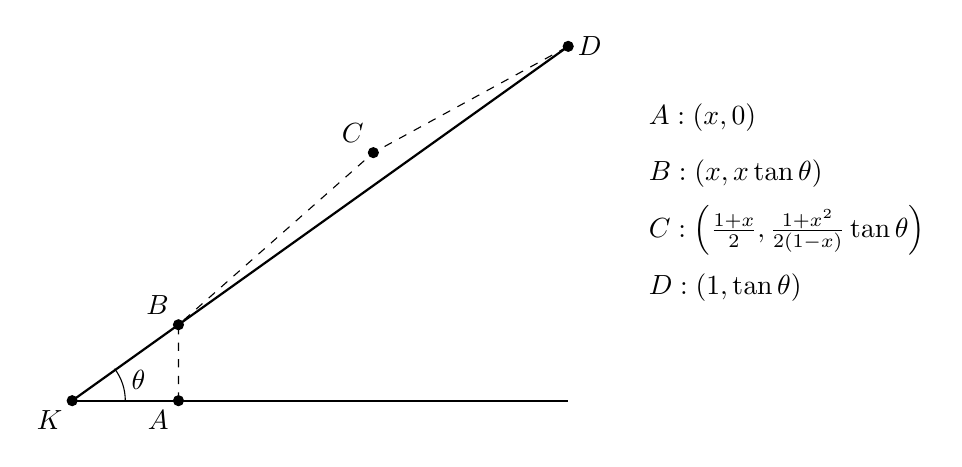
\begin{tikzpicture}[scale=0.9]
            \draw[thick] (0,0) -- (7,0);
            \draw[thick] (0,0) -- (7,5);
            \draw (0.75,0) arc (0:37:0.75);
            \draw (0.7,0.3) node[anchor=west] {$\theta$};
            \filldraw (3/2,0) circle (2pt) node[anchor=north east] {$A$};
            \filldraw (3/2,15/14) circle (2pt) node[anchor=south east] {$B$};
            \filldraw (17/4,3.5) circle (2pt) node[anchor=south east] {$C$};
            \filldraw (7,5) circle (2pt) node[anchor=west] {$D$};
            \filldraw (0,0) circle (2pt) node[anchor=north east] {$K$};
            \draw[dashed] (3/2,0) -- (3/2,15/14) -- (17/4,3.5) -- (7,5);
            \draw (8,4) node[anchor=west] {$A: (x,0)$};
            \draw (8,3.2) node[anchor=west] {$B: (x,x\tan\theta)$};
            \draw (8,2.4) node[anchor=west] {$C: \left(\frac{1+x}{2},\frac{1+x^2}{2(1-x)}\tan\theta\right)$};
            \draw (8,1.6) node[anchor=west] {$D: (1,\tan\theta)$};
        \end{tikzpicture}
        \caption{Shortening a line segment}\label{fig:shortline}
    \end{center}
\end{figure}

    Note that by choosing the coordinates above, we maintain that the area of $\Delta KAB$ matches the area of $\Delta BCD$, and thus, $|S| = |S'|$. Now we need to measure $P(S') = |AB| + |BC| + |CD|$.
    \begin{align*}
        |AB| &= x\tan \theta \\
        |BC| &= \frac{\sqrt{(3x^2-2x+1)^2 \tan^2\theta + (1-x)^4}}{2(1-x)} \\
        |CD| &= \frac{\sqrt{(x^2 + 2x - 1)^2\tan^2\theta + (1-x)^4}}{2(1-x)}
    \end{align*}
    Note that when $x=0$, we have that $P(S') = P(S) = \sec \theta$. Also, we have
    \[
        \frac{\partial P(S')}{\partial x}\Bigg|_{x=0} =\  \sec\theta (\sin\theta - 1).
    \]
    This quantity is negative for all acute angles $\theta$.  {\color{blue} Compactness of $\partial S$ implies $\partial S'$ does not intersect any other components of $\partial S$ for all sufficiently small values of $x$.}  Thus, for all sufficiently small values of $x$, we have  $P(S') < P(S)$.

   
\end{proof}

{\color{blue}
At a convex corner of $Q$, and curve $\partial S$ touching this corner makes an acute angle with at least one side.  Thus, we have the following corollary.

\begin{corollary}If $Q$ is a polygonal region and $S$ is an isoperimetric minimizer, then $\partial S$ cannot intersect any convex corner of $Q$.
\end{corollary}

We next focus on non-convex corners.  Momentarily believing Theorem \ref{thm:iso}, it follows that an isoperimetric minimizer \textit{can} intersect a non-convex corner of a region.  The next proposition shows that it cannot have two or more smooth boundary components which intersect a non-convex corner.

\begin{proposition} If $Q$ is a polygonal region and $S$ is an isoperimetric minimizer, then for each non-convex corner of $Q$, at most one smooth component of $\partial S$ can intersect it.

\end{proposition}

\begin{proof}
Assume for a contradiction that this fails and suppose $\partial S$ has at least two components, $\partial S_i$, $i=1,2,...$ touching a non-convex corner.

By Proposition \ref{prop:acuteCorner}, each $\partial S_i$ makes a right or obtuse angle with the sides of the corner of $Q$.  It follows that any two $\partial S_i$ make a convex angle.  Now, suppose that $\partial S_1$ and $\partial S_2$ are chosen so that no other $\partial S_i$ lie between them.  And assume initially those both $\partial S_1$ and $\partial S_2$ are line segments.


To bootstrap to this case where at least one of $\partial S_1$ and $\partial S_2$ are circular arcs, we apply the same argument used at the end of the proof of Proposition \ref{prop:acuteCorner}.

Thus, we can replace $S$ with a new region $S'$ with the same area but smaller perimeter and with two fewer smooth components touching this non-convex corner.  But induction, we may reduce until there are $0$ or $1$ touching the non-convex corner.
\end{proof}

}

\begin{proposition}
    Let $Q \subseteq \mathbb{R}^2$ be a polygonal region with $S \subseteq Q$, and let $Q$ contain a corner $K$. Let $U$
\end{proposition}

\begin{figure}
    \centering
    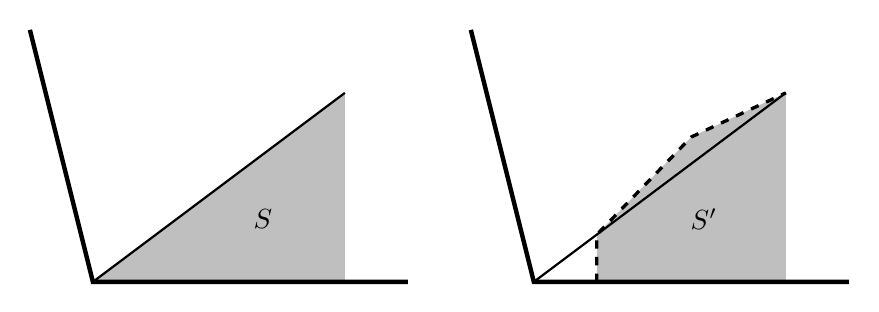
\begin{tikzpicture}[scale=0.8]
        \fill[color=gray!50] (0,0) -- (4,3) -- (4,0) -- cycle;
            \draw[ultra thick] (5,0) -- (0,0) -- (-1,4);
            \draw (2.7,1) node {$S$};
            \draw[thick] (0,0) -- (4,3);
        \begin{scope}[shift={(7,0)}]
            \fill[color=gray!50] (1,0) -- (1,0.75) -- (2.5,2.3) -- (4,3) -- (4,0) -- cycle;
            \draw[ultra thick] (5,0) -- (0,0) -- (-1,4);
            \draw (2.7,1) node {$S'$};
            \draw[thick] (0,0) -- (4,3);
            \draw[very thick, dashed] (1,0) -- (1,0.75) -- (2.5,2.3) -- (4,3);
        \end{scope}
    \end{tikzpicture}
    \caption{Deforming $S$, which touches a corner in an acute angle, to $S'$ so that it has the same area with a smaller perimeter while leaving the corner.}
    \label{fig:acuteCornerDeform}
\end{figure}


The next proposition deals with a single circular arc touching a corner $C$.  We distinguish the two sides of the corner depending on how the circle bends.  Specifically, the circular arc lies on one side of the tangent line to the circular arc at $C$.  The \textit{main side} of the corner is the side which does not lie on the same side of the tangent line as the circular arc.


We lastly address the special case where $S$ contains exactly two smooth components which intersect a corner $C$, at least in the case where at least one of them is a circular arc.

\begin{proposition}\label{prop:twocorners}Suppose $Q\subseteq \mathbb{R}^2$ is any polygonal region and suppose $S\subseteq Q$ is an isoperimetric minimizer for which $\partial S$ contains a circular arc touching a corner $C$ of $Q$.  If there are exactly two smooth component of $\partial S$ containing $C$, then the angle at $C$ between the circular arc and the main side cannot be acute.

\end{proposition}

\begin{proof}  Supposing there is such a pair of curves, we find a new region $S'$ with $A(S) = A(S')$ but $P(S') < P(S)$.   As in the proof of Proposition \ref{prop:onecorner}, we work in a small neighborhood of $C$ in which only the two hypothesized boundary curves of $\partial S$ appear in the neighborhood.  We replace a portion of the first curve with a line segment interpolating between a secant line and a tangent line at some point $T$ on the first curve.  If none of the line segments intersect the other curve, then the proof of Proposition \ref{prop:onecorner} works to prove this proposition.

By further shrinking the neighborhood if necessary, we can guarantee that the line segments have no intersections unless one of two things occurs: a) the second curve lies between the first curve and the main side or b) the two curves are tangent to each other.

Suppose a) occurs.  Then we modify the proof as follows: instead of having line segments begin at $T$ and end at a side of $Q$, we have them end on the other curve (at a point $T'$, depending on the slope of the line segment) and we use the new enclosed region.  Then using the secant line overestimates the area if and only if using the tangent line underestimates it.  By continuity, we particular line segment must yield precisely the same area.  And since we are shortening both curves, we have $A(S) = A(S')$ and $P(S' ) < P(S)$.

Thus, we may assume that a) does not occur and that b) does occur.  In this case, the tangent line at $T$ to the first curve does not intersect the second, but the secant line does in two points.

Given a line segment interpolating between the tangent line and secant line, which does not intersect the second or is tangent to it,  we create the new region $S'$ by using the entire second curve and replacing a portion of the first curve by the line segment.  On the other hand, if the line segment intersects the second curve in two points, we create $S'$  by following the segment from $T$ until it intersects the second curve, then following the second curve until it hits the second curve, then following the line segment will it hits a side of $Q$.

Using the tangent line is an overestimate of area if and only if using the secant line is an underestimate of area, so by continuity, we can select $S'$ with $A(S') = A(S)$.  But we also have $P(S') < P(S)$.
\end{proof}

If a corner forms an internal angle of $\pi/2$, i.e., it is a right angle, then no circular arc can be tangent to the non-main side while remaining in $Q$.  So, a circular arc makes a positive angle with the non-main side.  It follows that it must make an acute angle with the main side.  In addition, for a connected region, at most two boundary curves can intersect a single corner.  Thus, we have the following corollary of Propositions  \ref{prop:onecorner} and \ref{prop:twocorners}.

\begin{corollary}\label{cor:nocornercurve} If $Q$ has a corner $C$ for which the internal angle is $\pi/2$ and $S$ is a connected isoperimetric minimizer, the no circular arc boundary curve of $S$ can intersect $C$.

\end{corollary}

If $C\in Q$ is a corner for which the internal angle is at most $\pi/2$, then any segment intersecting $C$ necessarily makes two acute angles with the sides emanating from $C$.  In particular, we have the following corollary.

\begin{corollary}  Suppose $Q\subseteq\mathbb{R}^2$ is a polygonal region and let $C$ and $C'$ be any two corners of $Q$ for which the internal angle is at most $\pi/2$.  Then no isoperimetric minimizer $S\subseteq Q$ contains a boundary component which is either a) a line segment connecting $C$ and $C'$ or b) exactly one circular smooth component touching $C$.

\end{corollary}

\fi






\iffalse 

We conclude this section with a result, valid for all measurable subsets of all Riemannian manifolds\footnote{{\color{blue} Is there a larger class of shapes we can write here?}} which gives a sufficient condition for the isoperimetric function for \text{connected} measurable subsets to be the isoperimetric function all measurable subsets.

\begin{proposition}\label{prop:connecttodisconnect} Suppose $f:[0,|Q|/2]\rightarrow \mathbb{R}$ is the isoperimetric profile for connected subsets.  Assume that $f$ is continuous, non-decreasing, and there is $b\in (0,|Q|/2)$ for which the following hold:

\begin{itemize}\item $f|_{[0,b)}$ is convex

\item  $f'(x) > f'(y) $ for all $x\in [0,b)$ and all $y\in (b,|Q|]$

\item  $f(b) > \frac{1}{2} f(|Q|)$.

\end{itemize}

Then all isoperimetric minimizers must be connected, so that $f$ is also the isoperimetric profile for all measurable subsets.

\end{proposition}

Before proving this, we will need a lemma.

\begin{lemma}\label{lem:connect} Suppose a continuous $f:[0,|Q|/2]\rightarrow \mathbb{R}$ satisfies $f(0) = 0$, that $f$ is piecewise continuously differentiable, and that for some $c\in (0,|Q|/2)$ the inequality $f'(x) > f'(y)$ holds for all $x\in [0,c)$ and all $y\in (c,|Q|]$.  Then for any $x\in [0,c)$ and $y\in [c,|Q|/2]$, $f$ satisfies $f(x+y) < f(x) + f(y)$.

\end{lemma}

\begin{proof}  Fix $y\in [b,|Q|]$ and consider a varying $t\in (0,b)$ with $t$ close to $x$.  Since $y \geq b$ and $t+y \in \operatorname{dom} f$, $b < t+y \leq |Q|$.  Thus, by assumption, $f'(t) > f'(t+y)$.  Then $\int_{0}^x f'(t) dx > \int_0^x f'(t+y)\; dt$, or $f(x) - f(0) > f(x+y) - f(y)$.  Since $f(0) = 0$ by hypothesis, we find $f(x) + f(y) > f(x+y)$.
\end{proof}

We now prove Proposition \ref{prop:connecttodisconnect}.

\begin{proof}  We first show that no region having precisely two components is an isoperimetric minimizer.  So, suppose for a contradiction that $S = S_1 \coprod S_2$ is an isoperimetric minimizer have precisely two components.  Let $t_i = |S_i|$.

Assume initially $t_1 < b$.  If $t_2< b$ as well, by convexity of $f$ on $[0,b)$, it follows that we may apply Lemma \ref{lem:connect} with $c = t_2$ to conclude that $f(t_1 + t_2) < f(t_1) + f(t_2)$.  Similarly, if $t_2\in [b,|Q|]$, we apply Lemma \ref{lem:connect} with $c = b$.

So, we may assume that both $t_1,t_2 \geq b$ with $t_1+t_2\leq |Q|$.  Then, since $f$ is non-decreasing, $$f(t_1) + f(t_2) \geq f(b) + f(b) > f(|Q|) > f(t_1 + t_2).$$

Thus, in all cases, we find $f(t_1 + t_2) < f(t_1) + f(t_2) \leq P(S_1) + P(S_2)$, so that $S$ is not an isoperimetric minimizer.

Having handled the case of two components, we now proceed to the case where $S$ has $k\geq 3$ components, with $k$ finite.  We prove it by induction.  Specifically we assume that for some $k\geq 2$ that whenever $t_1,..., t_k$ are chosen in $(0,|Q|)$ in such a way so that $\sum_{i=1}^k t_i \in (0, |Q|)$, that $f\left( \sum_{i=1}^k t_i\right) < \sum_{i=1}^{k} f(t_i)$.   Our goal is to show that this holds with $K$ replaced by $K+1$.  So, select $k+1$ elements $t_1,..., t_{k+1}\in (0,|Q|)$ with $\sum_{i=1}^{k+1} t_i < |Q|$.

Then \begin{align*} f\left(\sum_i t_i\right) &= f\left(t_1 + \sum_{i=2}^{k+1} t_i\right)\\
&< f(t_1) + f\left(\sum_{i=2}^{k+1} t_i\right)\\
& < f(t_1) + \sum_{i=2}^{k+1} f(t_i)\\
&= \sum f(t_i).\end{align*}

This completes the inductive step, so we conclude that no region with finitely many components is an isoperimetric minimizer.

We now show that no isoperimetric minimizer exists with infinitely many components.  Consider the case where $S$ is a disjoint union of countably many components $S_i$, having $t_i = A(S_i)$.  We first prove that $f(\sum_i t_i) \leq \sum_i f(t_i)$.

Indeed, for any fixed integer $N$, we have $f\left(\sum_{i=1}^N t_i\right) < \sum_{i=1}^N f(t_i)$.  Taking the limit of both sides, we find $\lim_{N\rightarrow\infty} f\left(\sum_{i=1}^N t_i\right) \leq \sum_{i=1}^\infty f_a(t_i)$ (in the extended real numbers).  Since $f$ is continuous, we may commute it with the limit, finding $f\left(\sum_i t_i\right) \leq \sum_i f(t_i)$.

We conclude by proving that the inequality is actually strict.

We have \begin{align*} f \left(\sum_i t_i\right) &= f\left(t_1 + \sum_{i=2}^\infty t_i\right)\\ &< f(t_1) + f\left(\sum_{i=2}^\infty t_i\right)\\ &\leq f(t_1) + \sum_{i=2}^\infty f(t_i)\\ &= \sum_i f(t_i).\end{align*}

\end{proof}
\fi

\section{\texorpdfstring{The isoperimetric profile of $Q_a$}{The isoperimetric profile of Qa}}\label{sec:allconnected}

For each $a\in [0,1)$, we let $Q_a := [0,1]^2 \setminus [0,a)^2$ be the unit square with a square of side length $a$ removed from the bottom left corner.  The goal of this section is to determine the isoperimetric profile for $Q_a$.  We begin by introducing four regions, each parameterized by the area $t$, which we label $S_1$, $S_2$, $S_3$, and $S_4$, see Figure \ref{fig:main}.

In Section \ref{sec:fat}, we introduce a technical lemma, Lemma \ref{lem:technical}, which will allow us to precisely define a function $f_a:[0,\tfrac{1}{2}|Q_a|]\rightarrow \mathbb{R}$, which we will eventually prove is the isoperimetric profile for $Q_a$.  In Section \ref{sec:Sconnected}, we use Lemma \ref{lem:technical} to prove that an isoperimetric minimizer must be connected and must have precisely one smooth boundary component. In Section \ref{sec:faiso}, we use Lemma~\ref{lem:technical} to show that $f_a$ is the relative isoperimetric profile for connected regions with precisely one smooth boundary component.  The proof of Lemma \ref{lem:technical} is postponed to Section~\ref{sec:IV}.

\iffalse\begin{center}
    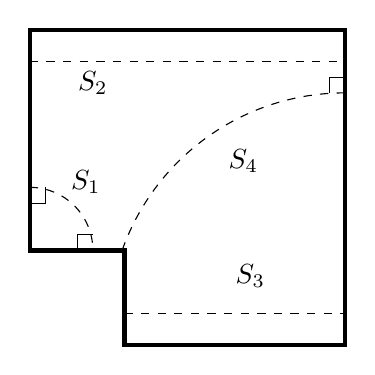
\begin{tikzpicture}[scale=4]
        \draw[ultra thick] (0.3,0) -- (1,0) -- (1,1) -- (0,1) -- (0,0.3) -- (0.3,0.3) -- cycle;
        \draw[dashed] (0,.9) -- (1,.9);
        \draw[dashed] (.3,0.1) -- (1,0.1);
        \draw[dashed] (1,0.8) arc (90:160:0.75);
        \draw (0,0.45) -- (.05,0.45) -- (0.05, .5);
        \draw (.15,.3) -- (.15,.35) -- (.2,.35);
        \draw[dashed] (0,.5) arc (90:0:.2);
        \draw (1,0.85) -- (0.95,0.85) -- (0.95,0.8);
        %\draw (0.29,0.15) node[anchor=east] {$a$};
        %\draw (0.65,0) node[anchor=north] {$1-a$};
        \draw (0.60,0.65) node[anchor=north west] {$S_4$};
        \draw (.1,.45) node[anchor = south west] {$S_1$};
        \draw (.2, .9) node[anchor = north] {$S_2$};
        \draw (.7, .15) node [anchor = south] {$S_3$};
    \end{tikzpicture}
    \captionof{figure}{Region $S_1$ is a quarter circle hitting boundary components of $Q_a$ perpendicularly.  Regions $S_2$ and $S_3$ are bounded by line segments of length $1$ and $1-a$ respectively, which parallel to the sides of $Q_a$.  Region $S_4$ is a portion of a circle connecting the nonconvex corner to a side of length 1, making a non-acute angle with both sides of $Q$ containing the nonconvex corner.}\label{fig:main}
\end{center}

\fi

\begin{center}
    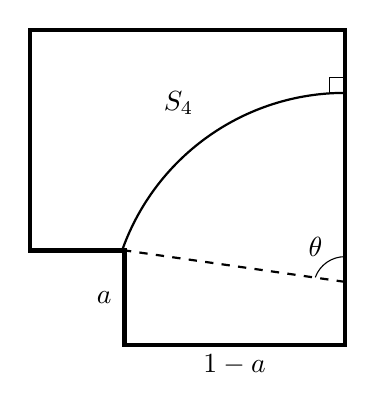
\begin{tikzpicture}[scale=4]
        \draw[ultra thick] (0.3,0) -- (1,0) -- (1,1) -- (0,1) -- (0,0.3) -- (0.3,0.3) -- cycle;
        \draw[thick,dashed] (1,0.2) -- (0.3,0.3);
        \draw[thick] (1,0.8) arc (90:160:0.75);
        \draw (1,0.85) -- (0.95,0.85) -- (0.95,0.8);
        \draw (1,0.28) arc (90:160:0.1);
        \draw (0.96,0.25) node[anchor= south east] {$\theta$};
        %\draw (0.6,0.25) node[anchor=south] {$R$};
        %\draw (1.01,0.1) node[anchor=west] {$s$};
        \draw (0.29,0.15) node[anchor=east] {$a$};
        \draw (0.65,0) node[anchor=north] {$1-a$};
        \draw (0.55,0.7) node[anchor=south east] {$S_4$};
    \end{tikzpicture}
    \captionof{figure}{One minimizing region}\label{fig:L}
\end{center}



We define four regions $S_1,S_2,S_3,$ and $S_4$ as follows.   The region $S_1$ is any region bounded by a quarter circle ending on sides of $Q_a$ orthogonally, except that we do not allow a quarter circle surrounding the non-convex corner.  The region $S_2$ is bounded by a line segment of length $1$.  The region $S_3$ is bounded by a line segment of length $1-a$.  And finally, the region $S_4$ is bounded by a curve which touches the nonconvex corner, intersects a wall of length 1 perpendicularly, and does not make an acute angle with either side of length $a$ at the nonconvex corner. For fixed $a$, such a region is characterized by a single angle $\theta$ and a choice of the wall of length $1$ it intersects, see Figure~\ref{fig:L}.  For concreteness in proofs, we will always assume an $S_4$ region touches the wall on the right, i.e., for fixed $a$, the notation $S_4(\theta)$ unambiguously describes a subset of $Q_a$.  We will eventually show that any minimizer is a region $S_i$ with $i\in \{1,2,3,4\}$.

\subsection{The isoperimetric profile}\label{sec:fat}

In this section, we begin with a technical lemma whose proof will be postponed to Section \ref{sec:IV}.

\begin{lemma}\label{lem:technical}  All the following hold:

\begin{enumerate}\item  There is a number $\theta_{max}\in (0,\tfrac{\pi}{2})$ with the property that for any $a\in [0,1)$ and for any $t\in \left[a(1-a), \frac{1}{2}(1-a^2)\right]$ there is a unique $\theta = \theta(t)\in [0,\theta_{max}]$ for which $|S_4(\theta)| = t$.

\item  For each fixed $a\in[0,1)$,  expressing $\theta$ in terms of $t$, we have $$\frac{d}{dt} P(S_4) = \frac{\sin \theta(t)}{1-a} > 0 \quad \text{and}\quad \frac{d^2}{dt^2}P(S_4) > 0$$ for all $t\in \left[a(1-a), \frac{1}{2}(1-a^2)\right].$

\item  For each fixed $a\in [0,1)$, $P(S_4) < \sqrt{2}(1-a)$ for all $t\in\left[a(1-a), \frac{1}{2}(1-a^2)\right]$.

\item  There is a value $t_0\approx 0.48$ which has the following property:  for any $t\in [0,t_0]$, there is a unique pair $(a(t),\theta(t))$ for which $|S_4| = t$ and $P(S_4) = 1$, but for any $t > t_0$ no such solution exists.  Moreover, $a(t)$ is a strictly increasing function of $t$.

\item  There is a number $\beta \approx 0.23$ for which $P(S_4) < 1$ for all $a \in (\beta,1)$ and all $t\in \left[a(1-a), \frac{1}{2}(1-a^2)\right]$.

\item  There are numbers $\alpha \approx 0.10$ and $\gamma = \frac{1}{1+\pi}$ with the property that for any $a\in [\alpha,\gamma]$, there is a unique area $t= \sigma(a)$ for which $P(S_4) = \sqrt{\pi |S_4|}$.

\item  For $a\in [\alpha,\gamma]$, $\sigma$ is a strictly decreasing function.  In addition, $\sigma(\alpha) = \frac{1}{\pi}$ and $\sigma(\gamma) = \frac{1}{\pi}(1-\gamma)^2$.  
\end{enumerate}

\end{lemma}

The precise definitions of $\alpha$ and $\beta$ are that $\alpha = a(\tfrac{1}{\pi})$ and $\beta = a(t_0)$ in the context of Lemma \ref{lem:technical}(4).  The function $\tau = \tau(a)$ is defined to be the inverse of the function $t\mapsto a(t)$, from Lemma \ref{lem:technical}(4).



In terms of these parameters, recalling that $\frac{1}{2}|Q_a| = \frac{1}{2}(1-a^2)$, we define the following continuous piecewise-smooth function $f_a:\left[0, \frac{1}{2}(1-a^2)\right]\rightarrow \mathbb{R}$.  Lemma \ref{lem:technical}(4) and (6) indicate that it is well-defined.

\begin{equation}\label{eq:profile}
       f_a(t)= \begin{cases}
            0 \leq a \leq \alpha & \begin{cases}
                (\pi t)^{1/2} & \hspace{4.9em}0\leq t \leq \frac{1}{\pi} \\
                1 & \hspace{4.6em}\frac{1}{\pi} \leq t \leq \frac{1}{2}(1-a^2)
            \end{cases} \\[2em]
            \alpha \leq a \leq \beta & \begin{cases}
                (\pi t)^{1/2} & \hspace{4.7em}0\leq t \leq \sigma \\
                P(S_4) & \hspace{4.6em}\sigma \leq t \leq \tau \\
                1 & \hspace{4.65em}\tau \leq t \leq \frac{1}{2}(1-a^2)
            \end{cases} \\[2em]
            \beta \leq a \leq \gamma & \begin{cases}
                (\pi t)^{1/2} & \hspace{4.7em}0\leq t \leq \sigma \\
                P(S_4) & \hspace{4.6em}\sigma \leq t \leq \frac{1}{2}(1-a^2) \\
            \end{cases} \\[2em]
            \gamma \leq a < 1 & \begin{cases}
                (\pi t)^{1/2} & \hspace{4.7em} 0\leq t \leq \frac{1}{\pi}(1-a)^2 \\
                1-a & \hspace{1em}\frac{1}{\pi}(1-a)^2 \leq t \leq a(1-a) \\
                P(S_4) & \hspace{1.7em}a(1-a) \leq t \leq \frac{1}{2}(1-a^2)
            \end{cases}
        \end{cases}
\end{equation}

The formulas appearing in $f_a$ are of the form $P(S_i)$ for some $i\in \{1,2,3,4\}$.  In particular, $f_a$ is an upper bound for the isoperimetric profile of $Q_a$.

The rest of Section \ref{sec:allconnected} is focused on proving the following result.

\begin{theorem}\label{thm:iso} For each $a\in [0,1)$, $f_a$ is the isoperimetric profile for $Q_a$.

\end{theorem}

We conclude this subsection with a lemma providing a useful upper bound for the function $f_a$. To state it, we let $T = T(a)$ denote the $t$-value at which $f_a$ transitions from $(\pi t)^{1/2}$ to a different formula.  Thus,
\[
    T(a) =
    \begin{cases}
        \frac{1}{\pi} & 0\leq a \leq \alpha \\
        \sigma (a) & \alpha \leq a \leq \gamma \\
        \frac{1}{\pi}(1-a)^2 & \gamma \leq a < 1
    \end{cases}.
\]
We also note that an $S_1$ region has area bounded by $\min\left\{\frac{\pi}{4}, \frac{\pi}{2}(1-a)^2\right\}$.  This follows because the largest such region occurs when it has $(1,1)$ as its center and the radius is bounded above by $\min\{1, \sqrt{2}(1-a)\}$ to avoid hitting both the walls of side length $1-a$ and the non-convex corner at $(a,a)$.




\begin{lemma}\label{lem:ffacts}For each $a\in [0,1)$ and any $t\in \left[0,\min\left\{\frac{\pi}{4}, \frac{\pi}{2}(1-a)^2\right\}\right]$ we have $$(\pi t)^{1/2} \geq f_a(t).$$  In addition, this inequality is strict for any $t> T$.

\end{lemma}

\begin{proof} 
We first observe that the function $(\pi t)^{1/2}$ has a negative second derivative on its domain.  On the other hand, the constant functions $1$ and $1-a$ and the function $P(S_4)$ have non-negative second derivatives with respect to $t$ on their domains, as follows from Lemma \ref{lem:technical}(2).

Set $h(t):=(\pi t)^{1/2} - f_a(t)$.  To complete the proof it is sufficient to show $h(t)\geq 0$ for $t\in \left[T,\frac{1}{2}(1-a^2)\right]$ with equality if and only if $t = T$.  Observe that $h$ is strictly concave. Thus, $\{t:h(t)\geq 0\}$ is an interval and the zeros of $h$ can only occur at the endpoints.

By definition of $T$, $h(T) = 0$.  Thus, we need only show $h(t_1) > 0$, where $t_1$ is the $t$-value corresponding to the largest possible area of $S_1$.  As mentioned above, $t\leq \min\left\{\frac{\pi}{4}, \frac{\pi}{2}(1-a)^2\right\}$. However, the area is also constrained by the domain of $f_a$, that is $\left[0,\frac{1}{2}(1-a^2)\right]$.  Since $\frac{1}{2}(1-a^2) < \pi/4$ for all $a\in[0,1)$, we find that $t_1 = \min \{ \frac{1}{2}(1-a^2), \frac{\pi}{2}(1-a)^2\}$, and hence $t_1 = \frac{1}{2}(1-a^2)$ when $a\leq \frac{\pi-1}{\pi+1}\approx 0.52$ and $t_1 = \frac{\pi}{2}(1-a)^2$ when $a\geq \frac{\pi-1}{\pi+1}$.   We consider two cases.


\textit{Case 1}: Assume $a\leq \frac{\pi-1}{\pi+1}$. If $a\leq \beta$, then $f_a(t_1)\leq 1$ and $\sqrt{\pi t_1} \geq \sqrt{\frac{\pi}{2}(1-\beta^2)}$. Thus, $$h(t_1) \geq \sqrt{\frac{\pi}{2}(1-\beta^2)} - 1 > 0.$$    On the other hand, if $a\in \left(\beta, \frac{\pi-1}{\pi+1}\right]$, then we must verify that $\sqrt{\pi t_1} - P(S_4)>0$.  By Lemma \ref{lem:technical}(3), we see $P(S_4) < \sqrt{2}(1-a)$.  In addition, it is easy to see that the minimum value of $h$ on $[\beta, \frac{\pi-1}{\pi+1}]$ occurs at $\beta$.  Therefore, $$h(t_1) > \sqrt{\frac{\pi}{2}(1-a^2)} - \sqrt{2}(1-a) \geq \sqrt{\frac{\pi}{2}(1-\beta^2)} - \sqrt{2}(1-\beta) > 0,$$ completing the case where $a\leq \frac{\pi-1}{\pi+1}$.

\textit{Case 2}: Assume $a> \frac{\pi-1}{\pi+1}$.  Then $$h(t_1) = \sqrt{\pi \frac{\pi}{2}(1-a)^2} - P(S_4) > \frac{\pi}{\sqrt{2}}(1-a) - \sqrt{2}(1-a) > 0,$$ completing this case.

\end{proof}









\iffalse

Our first step towards proving Theorem \ref{thm:iso} is to reduce to checking connected regions.

\begin{proposition}Suppose $f_a(t)$ is the isoperimetric profile for connected subsets of $Q_a$. Then it is the isoperimetric profile for $Q_a$.

\end{proposition}

\begin{proof}We verify the conditions of Proposition \ref{prop:connecttodisconnect}.  First, we showed in Proposition \ref{prop:derivativebounds} that $\frac{dP}{dt} > 0$, which implies that $f_a$ is non-decreasing.

Now, we take $b$ to be $T$.  Then since $(\pi t)^{1/2}$ is concave, the first bullet point holds.  So we now prove that $f'(x) > f'(y)$ for all $x\in [0,b)$ and $y\in \left(b,\frac{1}{2}(1-a^2)\right)$.

 To see this, we observe the smallest value of $((\pi t)^{1/2})' = \frac{\sqrt{\pi}}{2\sqrt{t}}$ occurs at the right end point.  From Lemma \ref{lem:sigmataubound} this right end point is at most $\frac{1}{\pi}$, yielding a derivative of $\pi/2 > 1$.  For $a\leq \gamma$, this estimate is sufficient: the derivative of a constant is $0 < \pi/2$ and the derivative of $P(\mathcal{L})$ is $\frac{\sin(\theta)}{1-a}\leq \frac{\sin(\theta)}{1-\gamma}\leq \frac{1+\pi}{\pi}\approx 1.31 < \pi/2$.

 For $a> \gamma$, we note that the right end point for the graph of $(\pi t)^{1/2}$ is $t = (1-a)^2/\pi$.  The derivative at this point is $\frac{\pi}{2(1-a)}$.  Since $\frac{\pi}{2} > 1$, $\frac{\pi}{2(1-a)} > \frac{1}{1-a} \geq \frac{\sin\theta}{1-a} = \frac{d}{dt}P(\mathcal{L})$.

\bigskip

We now verify the third condition, that $2f_a(b) > f_a\left(\frac{1}{2}(1-a^2)\right)$.   In all cases, $f(b) \geq 1-a$ since the corresponding curve connects two sides whose minimal distance is $1-a$, so $f(b) \geq 2(1-a)$.  We now argue that $f\left( \frac{1}{2}(1-a^2)\right) \geq \sqrt{2}(1-a)$, completing the proof of $3$.

 When $a\leq \beta$, $\sqrt{2}(1-a)\geq \sqrt{2}(a-\beta) \approx 1.07 > 1$.  Since $\max f_a(t) =1$ for $a\leq \beta$, the claim is established in this case.

Thus, we assume that $a > \beta$.  In this case, $f_a\left( \frac{1}{2}(1-a^2)\right) = P(a,\theta_{max})$.  From Lemma \ref{lem:PLmax}, we have $f_a\left( \frac{1}{2}(1-a^2)\right)\leq \sqrt{2}(1-a) < 2(1-a)$.


\end{proof}

\fi

\subsection{\texorpdfstring{The region $S$ must be connected}{The region S must be connected}}\label{sec:Sconnected}

In this section, we show that for an isoperimetric minimizer $S\subseteq Q_a$, the boundary $\partial S$ consists of exactly one smooth boundary component.  In particular, this implies that any minimizer must be connected.

 Recall that from Theorem \ref{thm:structure}, all smooth boundary components must have the same curvature.  Hence, either all smooth boundary components are line segments, or they are all arcs of circles of the same radius.  We begin with the case where they are line segments.

\begin{proposition}  If $S\subseteq Q_a$ is an isoperimetric minimizer for which all smooth boundary components of $\partial S$ are line segments, then there is only one smooth boundary component.
\end{proposition}

\begin{proof}  Suppose for a contradiction that $\partial S$ has at least two smooth line segment components.  Thus, $P(S) \geq 2(1-a)$. However, by Lemma \ref{lem:technical}(3), this is longer than $\max f_a$ when $a> \beta$, and longer than $1 = \max f_a$ when $a\leq \beta$.  Hence, $S$ is not an isoperimetric minimizer.
\end{proof}


We next move to the case where all smooth boundary components are arcs of a circle of radius $r$.  To that end, note that if such a smooth boundary component touches the nonconvex corner and it does not make an acute angle with either side, then one of three possibilities occurs:  it touches a side of length $a$ (so, must be a semicircle), it touches a side of length $1-a$ (so, it must be between quarter and half of a circle), or it touches a side of length 1 (so it bounds an $S_4$ region). The following lemma will be the key to handling the second case.

\begin{lemma}\label{lem:secondcase}
Suppose a circular segment of radius $r$ touches the non-convex corner in a non-acute angle and intersects a side of length $1-a$ perpendicularly.  Then $P\geq \sqrt{\pi t}$ where $P$ denotes the perimeter and $t$ denotes the area enclosed.
\end{lemma}

\begin{proof}
Suppose $\theta\in [\tfrac{\pi}{2},\pi]$ is the angle made by the endpoints of the circular segment and the center.  Then the area $t$ is given by $t = \tfrac{1}{2} r^2\theta -\tfrac{1}{2} r^2\cos\theta \sin\theta$ and the perimeter is $P = r\theta$.

Our goal is to show that $r\theta \geq \sqrt{\pi t}$, or, equivalently, that $\theta^2 \geq \frac{1}{2} \pi \theta - \frac{1}{2}\pi \cos\theta\sin\theta$.  Observe that when $\theta = \tfrac{\pi}{2}$, the inequality becomes the equality $\frac{\pi^2}{4} = \frac{\pi^2}{4}$.  Thus, it is sufficient to show the derivative of the left side is at least as large as the derivative of the right side for all $\theta \in [\tfrac{\pi}{2},\pi]$. The left side has derivative $2\theta \geq \pi$ on $[\tfrac{\pi}{2},\pi]$. On the other hand, the right side has derivative $\frac{1}{2}\pi - \frac{1}{2}\pi (\cos^2\theta - \sin^2\theta) = \pi \sin^2\theta$, which is bounded above by $\pi$ on $[\tfrac{\pi}{2},\pi]$.

\end{proof}

We are ready handle the case where all boundary components are arcs of a circle.

\begin{proposition} If $S\subseteq Q_a$ is an isoperimetric minimizer for which all smooth boundary components of $\partial S$ are cicular arcs of some radius $r$, then there is only one smooth boundary component.
\end{proposition}

\begin{proof} Suppose for a contradiction that $\partial S$ has at least two components and that all components have the same radius $r$. If the region $S$ lies inside one circular component and outside another, then by shrinking both at appropriate rates, the perimeter decreases while the area stays constant, contradicting minimality of $S$.  Thus, by replacing $S$ with its complement, we may assume without loss of generality that $S$ lies inside all of the circular components of its boundary.


Now, assume that no smooth boundary component bounds an $S_4$ region.  For a quarter, semi, or full circle, the length of the corresponding curve is at least $\sqrt{\pi t_i}$, where $t_i$ is the area enclosed by the $i$-th smooth boundary component.  For a curve touching the non-convex corner, it cannot make an acute angle with either side, by Theorem \ref{thm:corner}. Hence, it is either a semicircle touching the side of length $a$ or it touches the side of length $1-a$. In the first case, we find that its length is at least $\sqrt{\pi t}$, and the same conclusion holds for the second case by Lemma \ref{lem:secondcase}. Thus, in all cases, the length of $\partial S_i$ is bounded below by $\sqrt{\pi t_i}$.  Then, using Lemma \ref{lem:ffacts}, we find that
 $$P(S)  \geq \sum_i \sqrt{\pi t_i}  > \sqrt{\pi \sum_i t_i} = \sqrt{\pi t} \geq f_a(t),$$ proving that $S$ is not an isoperimetric minimizer.

It remains to consider the case where $\partial S$ contains a curve bounding an $S_4$ region. Such a curve has radius larger than or equal to $1-a$.  Observe that a quarter circle with radius larger than or equal to $1-a$ has perimeter at least $\frac{\pi}{2}(1-a)$.  Thus, an $S_4$ region with any other circular arc has perimeter at least $(1-a) + \frac{\pi}{2}(1-a) > \sqrt{2}(1-a)$.  From Lemma \ref{lem:technical}(3), this is larger than $\max f_a$ when $a\geq \beta$; and when $a < \beta$, $\sqrt{2}(1-a) > 1$, which is larger than $\max f_a$. 


\end{proof}


\subsection{\texorpdfstring{Showing that $f_a$ is the isoperimetric profile}{Showing fa is the isoperimetric profile}}\label{sec:faiso}

In this section, we complete the proof of Theorem \ref{thm:iso}.  By the results of Section \ref{sec:Sconnected}, we already know that all isoperimetric minimizers are connected with exactly one smooth boundary component. Our first goal will be to show that minimizer must be a region of type $S_1,S_2,S_3$ or $S_4$. 

\begin{proposition}\label{prop:ruleoutlots}Suppose $S$ is an isoperimetric minimizer.  Then $S$ must be one of the regions $S_1,S_2,S_3,$ or $S_4$.
\end{proposition}

\begin{proof}We already know that $S$ must be connected with a single smooth boundary component.  We know from Theorem \ref{thm:corner} that $\partial S$ cannot intersect any corner of $Q_a$, except possibly the non-convex corner.  We also know from Theorem \ref{thm:structure} that $\partial S$ has constant curvature, hence, it is a line segment or a portion of a circle, and that any intersections between $\partial S$ and $\partial Q$ are orthogonal, except possibly if they intersect at the nonconvex corner.   In particular, if $\partial S$ is a line segment, then it is an $S_2$ or $S_3$ region. Thus, for the rest of the proof, we assume that $\partial S$ is an arc of a circle.

If $\partial S$ is a full circle or semicircle of area $t$, then $P(S) > \sqrt{\pi t} \geq f_a(t)$. Therefore, $S$ is not a minimizer. Thus, we may assume that either $\partial S$ is a quarter circle or that it touches the non-convex corner.

\textit{Case 1}:  $S$ is quarter circle.  Then $S$ is an $S_1$ region except when it is a quarter circle surrounding the non-convex corner. Assume it surrounds the non-convex corner. If there is a region of type $S_1$, which has the same area as $S$, then it has smaller perimeter than $S$, which would contradict minimality.  

If $a\in \left[0, 1 - \frac{\sqrt{2}}{\pi}\right]$, the largest quarter circle of type $S_1$ we can fit in $Q_a$ has radius $1$. By continuity, we can find a region of type $S_1$ with $|S_1| = |S|$, showing $S$ is not minimal.

If $a\in \left(1 - \frac{\sqrt{2}}{\pi},1\right)$, since $P(S) = \sqrt{\pi(t + a^2)}$, we see that $P(S)\geq \sqrt{\pi}a$. As $\pi > 2$ and $a > 1-a$ for $a > 1-\frac{\sqrt{2}}{\pi} \approx 0.54$, we have $P(S) \geq \sqrt{\pi} a > \sqrt{2} (1-a)$.  Finally, since $1-\frac{\sqrt{2}}{\pi} > \gamma$, we conclude that $P(S) >   \max f_a$, by Lemma \ref{lem:technical}(3). This contradicts minimality of $S$ and completes the first case.

\textit{Case 2}:  $S$ touches the non-convex corner.  We assume that $\partial S$ is a portion of a circle touching the non-convex corner of $Q_a$ and no other corner.  If the other end point of $\partial S$ is on a wall of length $a$, then $\partial S$ is a half-circle, so it is not a minimizer.  If it is on the wall of length $1$, it is an $S_4$ region.  Finally, if the other endpoint of $\partial S$ is on a wall of length $1-a$, then we reflect it as in Figure \ref{fig:reflection}, to obtain a new region $S'$ of area $t$ and with $|\partial S'| = |\partial S|$.  Then $\partial S'$ touches a wall of length $1-a$ and a wall of length $1$.  If it hits the wall of length $1$, it is a quarter circle, hence a region of type $S_1$.  If it does not hit perpendicularly, then $S'$ is not a minimizer by Theorem \ref{thm:structure}.

\begin{center}
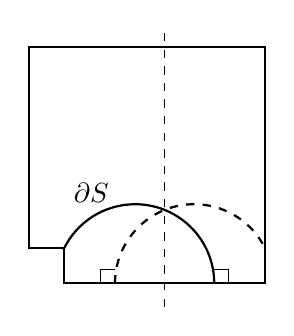
\begin{tikzpicture}[scale=3]
                \draw[thick] (0,1)  -- (1,1)  -- (1,0)  -- (0.15,0)  -- (0.15,0.15)  -- (0,0.15)  -- cycle;
                \draw[thick] (0.785,0) arc (0:155:0.335);
                \draw[thick,dashed] (0.365,0) arc (180:30:0.335);
                \draw[dashed] (0.575,-0.1) -- (0.575,1.08);
                \draw (0.15,0.3) node[anchor=south west] {$\partial S$};
                \draw (0.305,0) -- (0.305,0.06) -- (0.365,0.06);
                \draw (0.845,0) -- (0.845,0.06) -- (0.785,0.06);
\end{tikzpicture}
\captionof{figure}{Reflecting the region}\label{fig:reflection}
\end{center}



\end{proof}


We now work towards completing the proof of Theorem \ref{thm:iso} by determining for each $a\in [0,1)$ and each $t\in \left(0,\frac{1}{2}(1-a^2)\right]$ which type of the admissible regions has the shortest perimeter.  We recall that $T = T(a)$ is defined to be the $t$-value at which the formula for $f_a$ transitions away from $\sqrt{\pi t}$.  The next proposition indicates that for any $a\in [0,1)$, $f_a(t)$ is the isoperimetric profile for all $t\leq T$.

\begin{proposition}\label{prop:fsmallt} For any $a\in [0,1)$ and any $t\in (0,T]$, $S_1$ regions are isoperimetric minimizers.  Moreover, they are the only minimizers, unless $t = T$.
\end{proposition}

\begin{proof}
%The region $S_1$ we consider here is the quarter circle centered at the corner $(1,1)$ with $|S_1| = t$. Then the radius $r$ of $S_1$ is $r=2\sqrt{\tfrac{t}{\pi}}$. The biggest radius for which $S_1\subseteq Q_a$ is $r=\min\{\sqrt{2}(1-a),1\}.$  Therefore, the largest area that the region $S_1$ can bound is $\min\{\tfrac{\pi(1-a)^2}{2},\tfrac{\pi}{4}\}$. We note that $\sqrt{2}(1-a)\leq 1$ when  $a\leq 1-\tfrac{1}{\sqrt{2}}\approx 0.29$; in particular, this holds if $a\leq \gamma$.  Thus, for $a\leq \gamma$, we can find an $S_1$ region of any area up to $\frac{\pi}{4} > \frac{1}{\pi}.$  Since $\frac{1}{\pi}\geq T$ by Lemma \ref{lem:technical}(7), we can find the desired $S_1$ region for all $t\in(0,T]$.  On the other hand, for $a > \gamma$, we need to find a type $S_1$ region of area $t=\frac{1}{\pi}(1-a)^2$, which thus has radius $r=\frac{2}{\pi}(1-a)$.  But since $\frac{2}{\pi} < \sqrt{2}$, we see that $r \leq \min \{1, \sqrt{2}(1-a)\}$, so that a region of type $S_1$ exists in this case as well.

By Proposition \ref{prop:ruleoutlots}, we only need to compare $S_1$ regions with $S_2,S_3,$ and $S_4$ regions.  

\textit{Case 1}: Comparison with $S_2$ regions. Since $T\leq \frac{1}{\pi}$ (by Lemma \ref{lem:technical}(7)), it follows that $P(S_1) < P(S_2) = 1$ when $t<T$.

\textit{Case 2}: Comparison with $S_3$ regions.  We begin with the assumption that $a\in [\gamma,1)$.  Then $T(a) = \frac{1}{\pi}{(1-a)^2}$.  Observe that when $t= T$, $P(S_1) = P(S_3)$, and hence $P(S_1) < P(S_3)$ for $t < T$.  Next, when $a\in [0,\gamma)$, we note that there is an $S_3$ region only when $t\leq a(1-a)$.  Since $a< \gamma$, it follows that $a(1-a) < \frac{1}{\pi}(1-a)^2\leq T$, by Lemma \ref{lem:technical}(7). 

In particular, the proof of the proposition is complete for $t\in (a(1-a), T]$, since there is no corresponding $S_3$ region; and, for $t\in(0, a(1-a)]$, we have $$P(S_1) = \sqrt{\pi t}  \leq \sqrt{\pi a(1-a)} <  1-a = P(S_3).$$

\textit{Case 3}: Comparison with $S_4$ regions. We consider three subcases:  $a\in[0,\alpha)$, $a\in[\alpha,\gamma]$, and $a\in (\gamma,1)$.  

When $a\in [0,\alpha)$, by Lemma \ref{lem:technical}(4), the $t$-value at which $P(S_4(t)) = 1$ is less than $1/\pi$. Hence $P(S_1) < P(S_4)$ at $t = 1/\pi = T$, completing the case where $a\in [0,\alpha)$.

Next, assume $a\in [\alpha,\gamma]$.  Then, by definition of $\sigma$, when $t= T$ it follows that $P(S_1) = P(S_4)$.  The proof in this subcase will be complete once we show $\frac{d}{dt} P(S_1) > \frac{d}{dt} P(S_4)$ for all $t < T$.   Lemma \ref{lem:technical}(2) implies that 
\begin{equation*}
\frac{d}{dt} P(S_4)  = \frac{\sin \theta}{1-a} \leq \frac{1}{1-\gamma}\approx 1.32\quad\textrm{and}\quad\frac{d}{dt} P(S_1) = \frac{\sqrt{\pi}}{2\sqrt{t}} \geq \frac{\sqrt{\pi}}{2\sqrt{T}}.
\end{equation*}
Since $\sigma\leq \frac{1}{\pi}$, by Lemma \ref{lem:technical}(7), we have that $\frac{d}{dt} P(S_1) \geq \frac{\sqrt{\pi}}{2\sqrt{\frac{1}{\pi}}} = \frac{\pi}{2} \approx 1.57$.  Thus, $\frac{d}{dt} P(S_1) > \frac{d}{dt} P(S_4)$ for all $t< T$.

Finally, we assume $a\in (\gamma,1)$.  We follow a similar strategy to the proof in the previous sub-case.  First, since $a > \gamma$ and since a region of type $S_4$ has perimeter at least $1-a$, we see that $P(S_1) < P(S_4)$ at $t= T$. We have $\frac{d}{dt} P(S_4)\leq \frac{1}{1-a}$.  Substituting $t = T = \frac{1}{\pi}(1-a)^2$ into $\frac{d}{dt} P(S_1)$, we get $\frac{\pi}{2}\cdot\frac{1}{1-a}$.  Thus, $\frac{d}{dt} P(S_1) > \frac{d}{dt} P(S_4)$ when $a > \gamma$ as well.



\iffalse e now compare the perimeters of $P(S_1)$ and $P(S_3)$ with $|S_1|=|S_3|=t$ for the values $t$ for which both regions are defined, i.e., where $0<t\leq \min(\tfrac{\pi(1-a)^2}{2},\tfrac{1}{\pi},a(1-a))$. We solve the equation $1-a=P(S_3)=P(S_1)=\sqrt{\pi t}$ to obtain $t=\tfrac{1}{\pi}(1-a)^2$; this is $T$ when $a\geq \gamma$.  If $t< \frac{1}{\pi}(1-a)^2$, then $P(S_1) < P(S_3)$ and if $t > \frac{1}{\pi}(1-a)^2$, then $P(S_1) > P(S_3)$. Therefore, 
\begin{equation*}
a(1-a)\leq \tfrac{1}{\pi}(1-a)^2\quad\Longrightarrow\quad P(S_1)\leq P(S_3).
\end{equation*}
We also note that $a(1-a)\leq \tfrac{1}{\pi}(1-a)^2$ exactly when $a\leq \tfrac{1}{1+\pi}$. We define
\begin{equation}
\gamma=\frac{1}{1+\pi}\approx 0.24145.
\end{equation}
If $a\geq \gamma$, then 
\begin{equation*}
\begin{cases}
\frac{1}{\pi}(1-a)^2 \leq t\leq a(1-a)\quad\Longrightarrow\quad P(S_3) < P(S_1),\\
0 < t < \frac{1}{\pi}(1-a)^2\quad\Longrightarrow\quad P(S_3)>P(S_1).
\end{cases}
\end{equation*}
We note $\tfrac{(1-a)^2}{\pi} < \min \{ \tfrac{1}{\pi},  \tfrac{\pi}{2(1-a)^2}\}$, so  $S_1$ is defined for all these values of $t$.

On the other hand, when $a>1$ there is a type $S_1$ region Moreover, the perimeter $P(S_1)$ when $|S_1|=t$ is $P(S_1)=\sqrt{\pi t}$. Since the isoperimetric profile function for the region $Q_a$ is bounded by $1$, we are only interested in the region $S_1$ as long as $P(S_1)\leq 1$, which is exactly when $t\leq \tfrac{1}{\pi}$. Since $\tfrac{1}{\pi}<\tfrac{\pi}{4}$, we have $t\leq\min(\tfrac{\pi(1-a)^2}{2},\tfrac{1}{\pi})$. We see that
\begin{equation}
\frac{\pi}{2}(1-a)^2=\frac{1}{\pi}\quad\textrm{when}\quad a=1-\frac{\sqrt{2}}{\pi}\approx 0.54984.
\end{equation}
Together, $S_1$ with $|S_1|=t$ is defined for
\begin{equation} 
\begin{cases}
0<t<\tfrac{1}{\pi} & \textrm{when }0<a\leq 1-\tfrac{\sqrt{2}}{\pi},\\
0<t<\tfrac{\pi(1-a)^2}{2} & \textrm{when }a\geq 1-\tfrac{\sqrt{2}}{\pi}.
\end{cases}
\end{equation} 


\fi

\end{proof}

We can now complete the proof that $f_a$ is the isoperimetric profile of $Q_a$.

\begin{proposition}For any $a \in [0,1)$ and any $t \in \left(T, \frac{1}{2}(1-a^2)\right]$, $f_a$ is the isoperimetric profile for $Q_a$.

\end{proposition}

\begin{proof}From Lemma \ref{lem:ffacts}, since $t > T$ by hypothesis, we do not need to consider $S_1$ regions.  It remains to compare $S_2,S_3$, and $S_4$ regions. There are $S_3$ regions  only when $t\leq a(1-a)$ and there are $S_4$ regions only when $t \geq a(1-a)$ (and when $t = a(1-a)$, an $S_3$ region is an $S_4$ region). Hence, there is no $t$ for which we can compare $S_3$ and $S_4$.  Thus, we need only compare regions of type $S_2$ with regions of type $S_3$ or $S_4$.  We also note that, as shown in the proof of Proposition~\ref{prop:fsmallt}, for $a\leq \gamma$ we do not need to consider $S_3$ regions, as there is always an $S_1$ region with with the same area but smaller perimeter.  We break into cases depending on the value of $a$.

\textit{Case 1}:  $a\in[0, \alpha]$.  In the proof of Proposition \ref{prop:fsmallt}, we showed that the perimeter of an $S_4 = S_4(t)$ region is $1$ for some $t < \frac{1}{\pi}$.  Since $\frac{d}{dt} P(S_4)  >0$ by Lemma \ref{lem:technical}(2), it follows that $1 = P(S_2) < P(S_4)$ for all $t > \frac{1}{\pi}$.

\textit{Case 2}:  $a\in(\alpha,\beta]$.  By definition of $\sigma$, $P(S_4) = P(S_1)$ at $t=\sigma$.  Since $\sigma < \frac{1}{\pi}$ by Lemma \ref{lem:technical}(7), $P(S_1) < 1$, so $P(S_4) < 1 = P(S_2)$ at $\sigma$.  As $P(S_4)$ is an increasing function of $t$ by Lemma \ref{lem:technical}(2), and $\tau$ is defined as the $t$-value at which $P(S_4) = 1$,  it follows that $P(S_4) < 1= P(S_2)$ for $t\in(T,\tau)$, and that $P(S_4) > P(S_2)$ for $t < \tau$.

\textit{Case 3}: $a\in(\beta, \gamma)$.  By Lemma \ref{lem:technical}(5), $P(S_4) < 1 = P(S_2)$ for all $t\in \left[0,\frac{1}{2}(1-a^2)\right]$ for which both are defined.  In particular, for $a\in (\beta,\gamma]$, there is an $S_4$ region with area $t$ for all $t \in [T, \frac{1}{2}(1-a^2)]$, so that no $S_2$ region is a minimizer when $a\in(\beta,\gamma]$.

\textit{Case 4} $a\in (\gamma,1)$.  Lemma \ref{lem:technical}(5) implies $P(S_4)< P(S_2)$ whenever they are both defined.  Hence, no $S_2$ regions are minimizers; and $S_3$ regions have a shorter perimeter than corresponding $S_2$ regions when $t\in [T,a(1-a)]$.

\end{proof}


\iffalse

\subsection{The Curve $S_4$}

The curve $\mathcal{L}$ is a portion of a circle hitting the concave corner of $Q_a$ and hitting the right wall of $Q_a$ perpendicularly.  Such a curve is uniquely determined by  $a$ and $\theta$.

An elementary geometric argument gives the following formulas for the perimeter and area bounded by $\mathcal{L}$.

\begin{proposition}The perimeter of $\mathcal{L}$ is given by $$P(\mathcal{L}) = \frac{(1-a)\theta}{\sin \theta}$$ and the area bounded under $\mathcal{L}$ is $$A(\mathcal{L}) = \frac{(1-a)^2\theta}{2\sin^2 \theta} - \frac{(1-a)^2}{2\tan \theta} + a(1-a).$$

\end{proposition}




{\color{gray}\begin{theorem}\label{thm:fconnectR1boundary}  The isoperimetric profile among connected regions with smooth connected boundary is given by (\ref{eq:profile}).


\end{theorem}

\begin{proof}

Let $a \in [0,1)$. Suppose $S$ is a minimizing connected region with a smooth connected boundary such that $|S| = t \leq \frac{1}{2}(1-a^2)$. By definition $|\partial S| \leq f_a(t)$. Thus, it suffices to show that $|\partial S| \geq f_a(t)$. Note that $\partial S$ touches the boundary in at most two points. Furthermore, from Lemma \ref{lem:corner_to_corner} and Corollary \ref{cor:nocornercurve}, we have that $|\partial S|$ never touches a convex corner. Finally, from Theorem \ref{thm:structure},  we have that $\partial S$ is a curve with constant mean curvature, i.e., a portion of a circle or line, and $\partial S$ intersects the boundary orthogonally. With all of this in mind, we will now split into cases which depend on where $\partial S$ intersects the boundary of $Q_a$.
\begin{itemize}
    \item \underline{$\partial S$ never touches the boundary}: If $\partial S$ touches no walls and no corners, then $S$ must be a circle, and we have
    \[
        |\partial S| = 2(\pi t)^{1/2} > (\pi t)^{1/2} \geq f_a(t).
    \]
    \item \underline{$\partial S$ touches the boundary at a single point}: 
    \[
        |\partial S| = 2(\pi t)^{1/2} > (\pi t)^{1/2} \geq f_a(t).
    \]
    \item \underline{$\partial S$ touches the boundary on the same wall}: If $\partial S$ touches one wall and no corners, then $S$ must be a half circle, and we have
    \[
        |\partial S| = (2\pi t)^{1/2} > (\pi t)^{1/2} \geq f_a(t).
    \]
    \item \underline{$\partial S$ touches the boundary on adjacent walls}: If $\partial S$ touches two adjacent walls and no corners, then we have two possibilities for $S$. Either $S$ is a quarter circle or a three-quarter circle. If $S$ is a quarter circle, then we have
    \[
        |\partial S| = (\pi t)^{1/2} \geq f_a(t).
    \]
    If $S$ is a three-quarter circle, then we have
    \[
        |\partial S| = (3\pi( t+a^2))^{1/2} > (\pi t)^{1/2} \geq f_a(t).
    \]
    If $\partial S$ touches the nonconvex corner, then $S$ must be touching one of the walls of length $(1-a)$ orthogonally. This again requires $S$ to be a quarter circle, and we have our result.
    \item \underline{$\partial S$ touches the boundary on walls 2 away}: Assume for now that $\partial S$ does not touch the nonconvex corner. Then without loss of generality, we have three possibilities for the wall lengths $\partial S$ touches.
    \begin{itemize}
        \item $\partial S$ touches walls of lengths $a$ and $1$:

        In this case the only possibility for $\partial S$ is a straight line. Thus, $|\partial S| = 1-a$. Furthermore, the geometry requires $t \in [0,a(1-a)]$. Assume that $0 < a \leq \gamma = \frac{1}{1+\pi}$. Then we have $\frac{1-a}{\pi} \geq \frac{1}{1+\pi}$. In other words, we have $a \leq \frac{1}{1+\pi} \leq \frac{1-a}{\pi}$. Multiplying through by $(1-a)$ gives us
        \[
             \frac{1}{\pi}(1-a)^2 \geq a(1-a) \geq t.
        \]
        Now using the fact that $(\pi x)^{1/2}$ is a non-decreasing function, we have
        \begin{align*}
            |\partial S| &= 1-a \\
            &= \left(\pi \frac{1}{\pi}(1-a)^2\right)^{1/2} \\
            &\geq (\pi t)^{1/2} \\
            &\geq f_a(t).
        \end{align*}

        Now assume that $\gamma < a < 1$. If $0 \leq t \leq \frac{1}{\pi}(1-a)^2$, then the same argument works. If $\frac{1}{\pi}(1-a)^2 < t \leq a(1-a)$, then $|\partial S| = f_a(t)$, and we have our result. Thus, the only case to check is if $a(1-a) < t \leq \frac{1}{2}(1-a^2)$. However, $t \in [0,a(1-a)]$. Therefore, this case is finished.
        \item $\partial S$ touches walls of lengths $(1-a)$ and $1$: 
        
        Again, the only possibility in this case is a straight line such that $|\partial S| = 1$.  As Lemma \ref{lem:maxf_a} implies  $f_a(t)$ is bounded by 1, this case is finished.
        
        \item $\partial S$ touches walls of lengths $a$ and $(1-a)$:

        This case is impossible because an arc of a circle cannot meet both of these walls orthogonally.
    \end{itemize}
    Finally there is the case when $\partial S$ touches the nonconvex corner and a wall of length 1. If $\partial S$ has zero curvature, that is a straight line, then that case was already considered. Thus, we can assume that $\partial S$ is the arc of a circle which meets a wall of length 1 orthogonally. If the curvature is positive, then clearly $t \leq a(1-a)$ and $|\partial S| \geq 1-a$. Again, this case was already considered. Hence, we can assume $\partial S$ is the arc of a circle with negative curvature, see Figure \ref{fig:L}. This means $t \in [a(1-a),\frac{1}{2}(1-a^2)]$.

     If $\beta \leq a < 1$, then $|\partial S| = f_a(t)$. Thus, we will assume that $0<a<\beta$.   If $\alpha\leq a\leq \beta$, then from convexity of $(\pi t)^{1/2} - P(\mathcal{L})$, we find that $|\partial S| > f_a(t)$ for $t\leq \sigma$.  In addition, $|\partial S| = f_a(t)$ for $t\in[\sigma,\tau]$, and from Proposition \ref{prop:derivativebounds},  $P(\mathcal{L})> 1$ for $t>\tau$.
     
     If $a\leq \alpha$, then Proposition \ref{prop:uniquea} implies that the area at which $P(a,t) = 1$ is smaller than the area at which $P(\alpha,t) = 1$.  As $P(\mathcal{L})$ is increasing as a function of $t$, it follows that when $t = 1/\pi$, $P(\mathcal{L}) > 1 = \max f_a(t)$.  Thus, $|\partial S| > f_a(t)$ in this case.

     
    \item \underline{$\partial S$ touches the boundary on walls 3 away}: If $\partial S$ touches walls 3 away, then the complement of $S$ touches walls 2 away. Since we have already considered these cases, we are finished.\footnote{{\color{blue} I am not convinced we can dispose of this case so quickly since the complement of $S$ has the same boundary $\partial S$.  Maybe I just don't understand the argument.}}

    {\color{blue} Here's another proof of this case}

    If $\partial S$ touches the left and bottom walls, the orthogonality implies it is $3/4$ of a circle, and this case has been handled above. Otherwise, up to reflective symmetry of $Q_a$, we may assume $\partial S$ touches the top wall and the vertical wall of length $a$.  In this case, orthogonality implies $\partial S$ is a quarter circle, which has already been handled.
\end{itemize}
\end{proof}

{\color{magenta}Here is another style of proof for Theorem \ref{thm:fconnectR1boundary} where the cases are split by the shape of the boundary. I'm also trying to be much more careful.}

\begin{proof}
    Let $a \in [0,1)$. Suppose $S$ is a connected region with $|S| = t \leq \frac{1}{2}(1-a^2)$ such that its relative boundary is minimized. For ease of notation we will refer to this relative boundary as $\partial S$. By assumption, $|\partial S| \leq f_a(t)$. Thus, it suffices to show that $|\partial S| \geq f_a(t)$. 
    
    From previous discussions, we have that $\partial S$ is either a portion of a straight line or a portion of a circle. Furthermore, we have that $\partial S$ intersects the boundary of $Q_a$ orthogonally (or on the nonconvex corner). With this in mind, we will now consider cases based on the shape and location of $\partial S$.
    \begin{enumerate}
        \item Assume that $\partial S$ is a straight line of length $1$.

        From Lemma \ref{lem:maxf_a}, $f_a(t) \leq 1$. Thus, we have
        \[
            |\partial S| = 1 \geq f_a(t).
        \]
        
        \item Assume that $\partial S$ is a straight line of length $1-a$.

        The geometry requires that $t \in [0,a(1-a)]$. Here we must split into two cases: either $0 < a \leq \gamma = \frac{1}{1+\pi}$, or $\gamma < a < 1$. If $0 < a \leq \gamma$, then we have $\frac{1-a}{\pi} \geq \frac{1}{1+\pi}$. In other words, we have $a \leq \frac{1}{1+\pi} \leq \frac{1-a}{\pi}$. Multiplying through by $(1-a)$ gives us
        \[
            \frac{1}{\pi}(1-a)^2 \geq a(1-a) \geq t.
        \]
        Now using the fact that the square root function is non-decreasing, we have
        \begin{align*}
            |\partial S| &= 1-a \\
            &= \left(\pi \frac{1}{\pi}(1-a)^2\right)^{1/2} \\
            &\geq (\pi t)^{1/2} \\
            &\geq f_a(t).
        \end{align*}

        If instead $\gamma < a < 1$, then we are in the final piece of the piecewise definition of $f_a(t)$. If $t \in \left[0,\frac{1}{\pi}(1-a)^2\right]$, then the previous argument works. If $t \in \left[\frac{1}{\pi}(1-a)^2,a(1-a)\right]$, then
        \[
            |\partial S| = 1-a = f_a(t).
        \]
        Since $t \in \left[0, a(1-a)\right]$, this case is finished.
        \item Assume that $\partial S$ is a whole circle.

        In this case we have two possibilities. Either $S$ is the region inside of the circle, or $S$ is the region outside of the circle. If $S$ is inside of the circle, then we have
        \[
            |\partial S| = 2(\pi t)^{1/2} \geq (\pi t)^{1/2} \geq f_a(t).
        \]
        On the other hand, if $S$ is on the outside of the circle, then the area on the inside of the circle, $t'$, is greater than or equal to $\frac{1}{2}(1-a^2)$. This results in the following inequality:
        \begin{align*}
            |\partial S| &= 2(\pi t')^{1/2} \\
            &\geq 2\left[\pi \left(\frac{1}{2}(1-a^2)\right)\right]^{1/2} \\
            &= \sqrt{2\pi}(1-a^2)^{1/2} \\
            &\geq \sqrt{2\pi}(1-a) \\
            &> \sqrt{2}(1-a) \\
            &\geq f_a(t).
        \end{align*}
        \item Assume that $\partial S$ is a three-quarter-circle.

        Similar to the first case, either $S$ is the region inside of the three-quarter-circle or the region outside the three-quarter-circle. If $S$ is inside, then we have
        \[
            |\partial S| = \sqrt3(\pi t)^{1/2} > (\pi t)^{1/2} \geq f_a(t).
        \]
        If $S$ is the region on the outside, then we have
        \begin{align*}
            |\partial S| &= \sqrt{3}(\pi t')^{1/2} \\
            &\geq \sqrt{3}\left[\pi \left(\frac{1}{2}(1-a^2)\right)\right]^{1/2} \\
            &= \sqrt{3\pi}(1-a^2)^{1/2} \\
            &\geq \sqrt{3\pi}(1-a) \\
            &> \sqrt{2}(1-a) \\
            &\geq f_a(t).
        \end{align*}
        \item Assume that $\partial S$ is a half-circle.

        Following the pattern, if $S$ is on the inside, then we have
        \[
            |\partial S| = \sqrt{2}(\pi t)^{1/2} > (\pi t)^{1/2} \geq f_a(t).
        \]
        If $S$ is on the outside, then we have $t' > \frac{1}{2}(1-a^2)$. This leads to the following:
        \begin{align*}
            |\partial S| &= \sqrt{2}(\pi t')^{1/2} \\
            &\geq \sqrt{2}\left[\pi \left(\frac{1}{2}(1-a^2)\right)\right]^{1/2} \\
            &= \sqrt{\pi}(1-a^2)^{1/2} \\
            &\geq \sqrt{\pi}(1-a) \\
            &> \sqrt{2}(1-a) \\
            &\geq f_a(t).
        \end{align*}
        
        
        \item Assume that $\partial S$ is a quarter-circle.

        If $S$ is the region on the inside of the quarter-circle, we actually have two cases to consider. Either the $a \times a$ notch is also on the inside of the quarter-circle, or not. If not, then we have
        \[
            |\partial S| = (\pi t)^{1/2} \geq f_a(t).
        \]
        If the notch is on the inside of the quarter-circle, then we have
        \[
            |\partial S| = \left(\pi(t+a^2)\right)^{1/2} \geq (\pi t)^{1/2} \geq f_a(t).
        \]
        
        If $S$ is the region on the outside of the quarter-circle, then the area $t$ can be fit inside of the quarter-circle with a perimeter smaller than $|\partial S|$. This contradicts $\partial S$ being a minimizer.
        
        \item Assume that $\partial S$ is a portion of a circle which intersects the nonconvex corner. We know from ?? that $\partial S$ cannot intersect $Q_a$ in a convex corner. Thus, it must intersect a wall of $Q_a$ orthogonally. If it intersects a wall of length $a$, then $\partial S$ is a half-circle, which has already been considered. Thus, we two cases to investigate. Either $\partial S$ intersects a wall of length $1-a$, or it intersects a wall of length $1$.

        First we will consider the case when $\partial S$ is a circular arc connecting the nonconvex corner to a wall of length $1-a$. Consider reflecting $\partial S$ so that the new arc intersects a wall of length $1$ and a wall of length $1-a$, see below.

        \begin{center}
            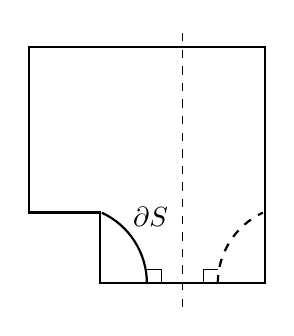
\begin{tikzpicture}[scale=3]
                \draw[thick] (0,1)  -- (1,1)  -- (1,0)  -- (0.3,0)  -- (0.3,0.3)  -- (0,0.3)  -- cycle;
                \draw[thick] (0.5,0) arc (0:65:0.33);
                \draw[thick, dashed] (0.8,0) arc (180:115:0.33);
                \draw (0.56,0) -- (0.56,0.06) -- (0.5,0.06);
                \draw (0.4,0.2) node[anchor=south west] {$\partial S$};
                \draw (0.74,0) -- (0.74,0.06) -- (0.8,0.06);
                \draw[dashed] (0.65,-0.1) -- (0.65,1.08);
            \end{tikzpicture}
            \hspace{5em}
            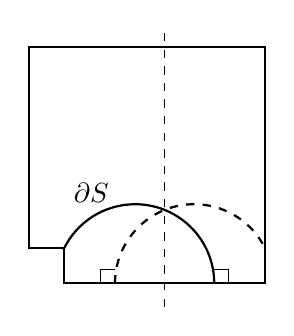
\begin{tikzpicture}[scale=3]
                \draw[thick] (0,1)  -- (1,1)  -- (1,0)  -- (0.15,0)  -- (0.15,0.15)  -- (0,0.15)  -- cycle;
                \draw[thick] (0.785,0) arc (0:155:0.335);
                \draw[thick,dashed] (0.365,0) arc (180:30:0.335);
                \draw[dashed] (0.575,-0.1) -- (0.575,1.08);
                \draw (0.15,0.3) node[anchor=south west] {$\partial S$};
                \draw (0.305,0) -- (0.305,0.06) -- (0.365,0.06);
                \draw (0.845,0) -- (0.845,0.06) -- (0.785,0.06);
            \end{tikzpicture}
        \end{center}
        Note that if this reflected curve intersects a wall of length $1$ non-orthogonally, then this contradicts $\partial S$ being a minimizer. If this reflected curve does intersect orthogonally, then $\partial S$ is a quarter-circle, which has already been considered.

        Next we will consider the case when $\partial S$ is a circular arc connecting the nonconvex corner to a wall of length $1$. First, consider the case when $\partial S$ is concave up, see below.

        \begin{center}
            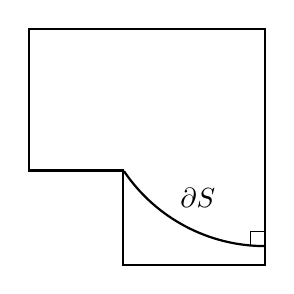
\begin{tikzpicture}[scale=3]
                \draw[thick] (0,1)  -- (1,1)  -- (1,0)  -- (0.4,0)  -- (0.4,0.4)  -- (0,0.4)  -- cycle;
                \draw[thick] (1,0.08) arc (270:214:0.72);
                \draw (0.6,0.2) node[anchor=south west] {$\partial S$};
                \draw (1,0.14) -- (0.94,0.14) -- (0.94,0.08);
            \end{tikzpicture}
        \end{center}

        Since $t$ is at most half of the area, $S$ must be the region below the arc. Thus, $t \leq a(1-a)$. We can bound this area with a straight line of length $1-a$, which is smaller than $\partial S$. This contradicts $\partial S$ being a minimizer.

        Lastly, we must consider $\partial S$ being an arc which is concave down, see below.

        \begin{center}
            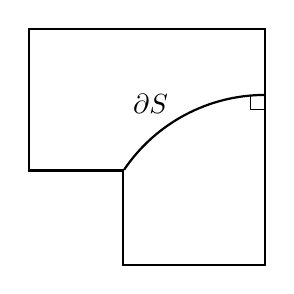
\begin{tikzpicture}[scale=3]
                \draw[thick] (0,1)  -- (1,1)  -- (1,0)  -- (0.4,0)  -- (0.4,0.4)  -- (0,0.4)  -- cycle;
                \draw[thick] (1,0.72) arc (90:146:0.72);
                \draw (0.4,0.6) node[anchor=south west] {$\partial S$};
                \draw (1,0.66) -- (0.94,0.66) -- (0.94,0.72);
            \end{tikzpicture}
        \end{center}

        If $S$ is the region above the arc, then more than half of the area is below the arc. Thus, we can fit an area of $t$ below the arc. We can then shrink $\partial S$ to bound this area. Again, this contradicts $\partial S$ being a minimizer. Therefore, we will assume $S$ is the region below the arc. Note that this forces $t \in \left[a(1-a),\frac{1}{2}(1-a^2)\right]$. ...unfinished...
    \end{enumerate}
\end{proof}

}

\fi


\section{A proof of Lemma \ref{lem:technical}}\label{sec:IV} In this section, we prove Lemma \ref{lem:technical}. We consider an $S_4$ region, which is determined by $a$ and $\theta$; hence we sometimes write $S_4(a,\theta)$. An elementary geometric argument gives the following formulas for the perimeter and area of $S_4$.

\begin{proposition}\label{prop:geo}The perimeter of $S_4 = S_4(a,\theta)$ is given by \begin{equation}\label{eqn:perim}P(S_4) = \frac{(1-a)\theta}{\sin \theta}\end{equation} and the area of $S_4$ is \begin{equation}\label{eqn:area}|S_4| = \frac{(1-a)^2\theta}{2\sin^2 \theta} - \frac{(1-a)^2}{2\tan \theta} + a(1-a).\end{equation}

\end{proposition}


Both equations \eqref{eqn:perim} and \eqref{eqn:area} have continuous extensions to $\theta = 0$ with $P(S_4) = 1-a$ and $|S_4| = a(1-a)$.  We will always use these extensions.



Recall that $|Q_a| = 1-a^2$. We are interested in $t\in (0, \tfrac{1}{2}(1-a^2)]$.  The following lemma indicates the domain of $\theta$ takes the form $[0,\theta_{max}]$, where $\theta_{max}$ is independent of $a$. The value of $\theta_{max}$ is approximately $1.21$.


\begin{lemma}\label{lem:thetamax}  The equation $|S_4| = \frac{1}{2}(1-a^2)$ admits a unique solution $\theta_{max}\in[0,\tfrac{\pi}{2}]$.

\end{lemma}

\begin{proof} The equation $|S_4| = \frac{1}{2}(1-a^2)$ is equivalent to the equation \begin{equation}\label{eqn:thetamax} 1 = \frac{\theta}{\sin^2\theta} - \frac{1}{\tan\theta}.\end{equation} As $\theta$ approaches $0$ and $\tfrac{\pi}{2}$, the right side of equation \eqref{eqn:thetamax} approaches $0 $ and $\tfrac{\pi}{2}$, respectively.  By the Intermediate Value Theorem, equation \eqref{eqn:thetamax} has a solution $\theta_{max}$.

The derivative of the right side of equation \eqref{eqn:thetamax} is $-2\csc^2 \theta \left(\theta \cot \theta-1\right)$.  We claim that $\theta\cot\theta-1 < 0$ on $(0,\frac{\pi}{2})$.  Indeed, this follows from the fact that its limiting value at $0$ is $0$ and that its derivative is $\frac{1}{\sin\theta}\left(\cos\theta - \frac{\theta}{\sin\theta}\right) < 0$.  Having established the claim, uniqueness of the solution to equation \eqref{eqn:thetamax} now follows.

\end{proof}

We now prove Lemma \ref{lem:technical}(1)


\begin{proposition}\label{prop:inverse} The number $\theta_{max}$ has the property that for any fixed $a\in [0,1)$ and for any $t\in \left[a(1-a), \frac{1}{2}(1-a^2)\right]$, there is a unique $\theta = \theta(t)\in [0,\theta_{max}]$ for which $|S_4(\theta)| = t$.

\end{proposition}

\begin{proof} To prove existence, we note that the formula for $|S_4|$ shows that it is continuous as a function of $\theta$ on $(0,\theta_{max})$.  Since its limit as $\theta$ approaches $0$ is $a(1-a)$ and its value at $\theta_{max}$ is $\frac{1}{2} (1-a^2)$, existence follows from the Intermediate Value Theorem.


For uniqueness, fixing $a$, we compute $\frac{d |S_4|}{d\theta} = \frac{dt}{d \theta} = \frac{(1-a)^2 (\sin\theta - \theta\cos\theta)}{\sin^3\theta}$.  We claim that this is positive on $(0,\theta_{max})$.  Indeed, the factor $\frac{(1-a)^2}{\sin^3 \theta}$ is positive and $\sin\theta - \theta\cos\theta$ is positive, because it has limiting value $0$ at $\theta = 0$ and derivative $\theta\sin\theta > 0$ on $(0,\pi)$.  As $\frac{d |S_4|}{d \theta}$ is positive, it follows that for fixed $a$, there is at most one solution to the equation $|S_4| =t$.
\end{proof}

In light of Proposition \ref{prop:inverse}, for fixed $a\in[0,1)$ and $\theta\in [0,\theta_{max}]$, the map $\theta\mapsto |S_4(\theta)|$ has an inverse.  When we write $S_4(t)$, we mean $S_4(\theta)$ precomposed with this inverse.  We now prove Lemma \ref{lem:technical}(2).

\begin{proposition}\label{prop:derivativebounds} For each fixed $a\in[0,1)$,  $\frac{d}{dt} P(S_4(t)) = \frac{\sin \theta(t)}{1-a} > 0$ and $\frac{d^2}{dt^2}P(S_4(t)) > 0$ for all $t\in \left[a(1-a), \frac{1}{2}(1-a^2)\right]$.

\end{proposition}

\begin{proof} The chain rule gives $\frac{d P(S_4(t))}{d t} = \frac{dP(S_4(\theta))}{d \theta} \cdot\frac{d\theta}{d t}$.  The first factor simplifies to $\frac{(1-a)(\sin\theta-\theta\cos\theta)}{\sin^2\theta}$ while the second factor is $\frac{1}{\frac{d t}{d \theta}} = \frac{\sin^3\theta}{(1-a)^2 (\sin\theta-\theta\cos \theta)}$.  Multiplying these together, we find that $\frac{d}{dt} P(S_4(t)) = \frac{\sin \theta}{1-a} > 0$, as claimed.

For the second derivative, the chain rule gives $\frac{d^2 P(S_4(t)) }{dt^2} = \frac{d}{d\theta}(\frac{dP(S_4(t))}{dt})\cdot \frac{d\theta}{dt}$.  The first factor is $\frac{\cos\theta}{1-a} > 0$ and the second factor is $\frac{1}{\frac{dt}{d\theta}}$, which is positive, by the proof of Proposition \ref{prop:inverse}.


\end{proof}


We now prove Lemma \ref{lem:technical}(3).

\begin{lemma}\label{lem:PLmax}For each fixed $a\in [0,1)$ and any $t\in\left[a(1-a), \frac{1}{2}(1-a^2)\right]$ we have that $P(S_4(t)) < \sqrt{2}(1-a)$. 

\end{lemma}

\begin{proof}Because $\frac{dP}{dt} = \frac{\sin\theta}{1-a} > 0$, the maximum value of $P(S_4(t))$ occurs when $t = \frac{1}{2}(1-a^2)$.  Because $\frac{d\theta}{dt} > 0$, this occurs when $\theta = \theta_{max}$.  Recalling that $\theta_{max}$ solves equation \eqref{eqn:thetamax}, we see that $\theta_{max}$ also solves the equation $\frac{\theta_{max}}{\sin\theta_{max}} = \sin\theta_{max} + \cos\theta_{max} = \sqrt{2}\sin\left(\tfrac{\pi}{4} + \theta_{max}\right)$.  Thus, $$P(S_4(t)) \leq (1-a) \frac{\theta_{max}}{\sin\theta_{max}}  = (1-a) \sqrt{2}\sin\left(\frac{\pi}{4} + \theta_{max}\right).$$  Since $\theta_{max}\in (\tfrac{\pi}{4},\tfrac{\pi}{2})$, $\sin(\tfrac{\pi}{4} + \theta_{max}) < 1$, so we find $P(S_4) < \sqrt{2}(1-a)$.

\end{proof}

We now prove Lemma \ref{lem:technical}(4).  We define $$t_0 = \frac{-2 \sin^2\theta_{max}+\left(2 \theta_{max} -\cos\theta_{max}\right) \sin\theta_{max}+\theta_{max}}{2 \theta_{max}^{2}}\approx 0.48.$$

\begin{proposition}\label{prop:uniquea} The number $t_0$ has the following property:  for any $t\in [0,t_0]$, there is a unique pair $(a(t),\theta(t))$ for which $|S_4(t)| = t$ and $P(S_4(t)) = 1$, but for any $t > t_0$ no such solution exists.  Moreover, $a(t)$ is a strictly increasing function of $t$. 

\end{proposition}

\begin{proof}
It is easy to see that $P(S_4)=1$ if and only if $a = 1-\frac{\sin\theta}{\theta}$. Hence, $\theta$ determines $a$ uniquely.  If we substitute this into equation \eqref{eqn:area}, we find that\begin{equation}\label{eqn:tintermsoftheta}t =\frac{-2 \sin^2 \left(\theta \right)+\left(2 \theta -\cos \theta \right) \sin\theta +\theta}{2 \theta^{2}}.\end{equation}

As $\theta$ approaches $0$, this expression limits to $0$, and at $\theta_{max}$ we obtain $t_0$.  Thus, existence of a solution for each $t$ in the interval follows from the Intermediate Value Theorem.

For uniqueness, we compute $$\frac{dt}{d\theta} = \frac{\left(\cos\! \left(\theta \right)+2 \sin\! \left(\theta \right)-\theta \right) \left(\sin\! \left(\theta \right)-\cos\! \left(\theta \right) \theta \right)}{\theta^{3}}.$$   Since both factors of the numerator are positive %\footnote{For the first factor, the second derivative is $-2\sin\theta - \cos\theta < 0$ on $\pi/2$, so the graph is concave down, so the minimum occurs at the end points.  At $0$ it has the value $1$ and at $\pi/2$, it has the value $2-\pi/2 > 0$, so it's positive on $(0,pi/2)$.  For the second factor, the derivative is $\theta\sin\theta > 0$ on $(0,\pi/2)$, so that factor is increasing on $(0,\pi/2)$.  At $\theta = 0$, it has the value $0$, so it is always positive on $(0,pi/2)$.  I don't know if this needs to be added to the article or not.}
on $(0,\theta_{max}]$, $\frac{dt}{d\theta}$ is strictly increasing. Thus, there is at most one solution to equation \eqref{eqn:tintermsoftheta}.  Moreover, since $\frac{dt}{d\theta} $ is positive, it follows that for any $t > t_0$, there is no solution to equation \eqref{eqn:tintermsoftheta} with $\theta\in(0,\theta_{max}]$, which in turn implies there is no solution to the system $P(S_4) = 1$, $|S_4| = t$.

We conclude the proof by showing that $a(t)$ is a strictly increasing function of $t$.  Assume $t_1 < t_2$ with both $t_1$ and $t_2$ in the interval and let $(a_1,\theta_1)$ and $(a_2,\theta_2)$ solve the above system with $t= t_1$ and $t=t_2$, respectively.   Then, from equation \eqref{eqn:tintermsoftheta} and from the fact that $\frac{dt}{d\theta} > 0$, we conclude that $\theta_1<\theta_2$.  Finally, from the equation $a = 1-\frac{\sin\theta}{\theta}$, we conclude that $a_1 < a_2$.


\end{proof}

We now obtain Lemma \ref{lem:technical}(5) as a corollary.  Recall that $\beta\approx 0.23$ is defined as $a(t_0)$ in the notation of the previous proposition.


\begin{corollary}The number $\beta$ has the property that $P(S_4(t)) < 1$ for all $a \in (\beta,1)$ and all $t\in \left[a(1-a), \frac{1}{2}(1-a^2)\right]$.
\end{corollary}

\begin{proof}
By definition, $t_0$ is the value obtained from equation \eqref{eqn:tintermsoftheta} when $\theta = \theta_{max}$. Hence, $\beta  =  1-\frac{\sin \theta_{max}}{\theta_{max}}\approx 0.23$. Equivalently, $\frac{(1-\beta)\theta_{max}}{\sin\theta_{max}} = 1$.  Then, for any $a > \beta$ and any $\theta \in (0,\theta_{max}]$, we see that $$P(S_4(a,\theta)) = \frac{(1-a)\theta}{\sin \theta} < \frac{(1-\beta)\theta_{max}}{\sin\theta_{max}} = 1.$$
\end{proof}


\iffalse

\begin{proposition} The number $\theta_\tau$ is unique so that $\tau$ is well-defined.

\end{proposition}

\begin{proof}  Fix $a\in[\alpha,\beta]$.  We have $P(a,\theta) = 1$ if and only if $\frac{\theta}{\sin\theta} = \frac{1}{1-a}$.  We claim there is a unique $\theta_\tau\in (0,\theta_{max})$ solving this equation.  Indeed the function $\frac{\theta}{\sin\theta}$ has derivative $(1-\theta\cos\theta)\csc\theta)$ which we have already argued is positive on $(0,\theta_{max})$.  Thus, this function is increasing, so there is at most one solution $\theta_\tau$ to $\frac{\theta_\tau}{\sin \theta_1\tau} = \frac{1}{1-a}$.

The value of $\frac{\theta}{\sin\theta}$ as $\theta$ approaches $0$ from the right is $1$.  The value at $\theta_{max}$ is $\beta$.  Since $a\leq \beta$, it follows that $\frac{1}{1-a}\leq \frac{1}{1-\beta} =\frac{ \theta_{max}}{\sin\theta_{max}}$.  Thus, by the Intermediate Value Theorem, $\theta_\tau$ exists.

\end{proof}

\fi


We now prove Lemma \ref{lem:technical}(6).  Recall that $\alpha\approx 0.1$ is defined to be $a(\tfrac{1}{\pi})$ in the notation of Proposition \ref{prop:uniquea}, while $\gamma = \frac{1}{1+\pi}\approx 0.24$.

\begin{proposition}\label{prop:sigmadefined} For any $a\in [\alpha,\gamma]$, there is a unique area $\sigma(a) = t$ for which $P(S_4(t)) = \sqrt{\pi |S_4(t)|}$.

\end{proposition}

\begin{proof}
Fix $\alpha \leq a\leq \gamma$.  Consider the function $j:[0,\theta_{max}]\rightarrow \mathbb{R}$ defined by \begin{equation}\label{eqn:j}j(\theta) = \frac{1}{1-a}\left(P^2(S_4) - \pi |S_4|\right).\end{equation}  Observe that a zero of $j$, when substituted into equation \eqref{eqn:area}, yields $\sigma(a)$. We compute that $j(0) = (1-a) - \pi a = (1-(\pi+1)a) \geq 0$, since $a\leq \gamma= \frac{1}{1+\pi}$. We claim that $j(\theta_{max}) < 0$ for $ a\geq \alpha$.  To see this, assume for a contradiction that $j(\theta_{max}) \geq 0$.  Solving this inequality for $a$, we find that $$a\leq -\frac{\pi\theta_{max} \tan  \theta_{max}  -2 \theta_{max}^{2} \tan\theta_{max}-\pi\sin^2 \theta_{max}}{2\pi \tan\theta_{max}  \sin^2 \theta_{max} -\pi\theta_{max}\tan \theta_{max} +2 \theta_{max}^{2} \tan\theta_{max}+\pi\sin^2 \theta_{max}}.$$  As the right side evaluates to approximately $0.03 < \alpha$, we have a contradiction.  By the Intermediate Value Theorem, for each $a\in [\alpha,\gamma]$, there is a number $\theta = \theta(a)$ for which $j(\theta) = 0$,  which gives $P(S_4(\theta)) = \sqrt{\pi |S_4(\theta)|}$. We claim that $\theta$ is unique.  Indeed, we have $$\frac{dj}{d\theta} = (1 - a) (\pi - 2 \theta) (-1 + \theta \cot\theta) \csc^2(\theta).$$ In the proof of Lemma \ref{lem:thetamax}, we showed $-1 + \theta\cot(\theta)$ is non-zero, and $\pi - 2\theta = 0$ if and only if $\theta = \frac{\pi}{2}$.  It follows that $\frac{dj}{d\theta}\neq 0$  on $[0,\theta_{\max}]$. Hence $j$ is injective.

\end{proof}

We conclude with a proof of Lemma \ref{lem:technical}(7).

\begin{lemma}\label{lem:sigmataubound}  For $a\in [\alpha,\gamma]$, $\sigma$ is a strictly decreasing function.  In addition, $\sigma(\alpha) = \frac{1}{\pi}$ and $\sigma(\gamma) = \frac{1}{\pi}(1-\gamma)^2$.  
\end{lemma}

\begin{proof}  We first claim that $\sigma(\alpha) = \frac{1}{\pi}$.  Indeed, by definition of $\alpha$, there is an angle $\theta_\alpha$ for which $|S_4(\alpha,\theta_{\alpha})| = \frac{1}{\pi}$ and $P(S_4(\alpha,\theta_{\alpha})) = 1$.  Observe that $P(S_4) = \sqrt{\pi |S_4|}$. Hence, by definition of $\sigma$, $\sigma(a) = \frac{1}{\pi}$.

We claim that $\sigma(\gamma) = \frac{1}{\pi}(1-\gamma)^2$.  To see this, observe that equation \eqref{eqn:area} is solved with $a = \gamma$ and $\theta = 0$.  Substituting these values into equations \eqref{eqn:perim} and \eqref{eqn:area}, we find that $P(S_4) = (1-\gamma)$ and $|S_4| = \gamma(1-\gamma) = \frac{1}{\pi}(1-\gamma)^2$.  Thus, $P(S_4)^2 = \pi |S_4|$, which implies $\sigma(\gamma) = |S_4| = \frac{1}{\pi}(1-\gamma)^2$.

Next, we show that $\sigma$ is a strictly decreasing function of $a$.   First, we use equation \eqref{eqn:j} with $j=0$ to define $\theta$ in terms of $a$.  We get that $$\frac{d\theta}{da} = -\frac{\frac{\partial j}{\partial a}}{\frac{\partial j}{\partial \theta}} = \frac{(-2\pi \sin^2\theta - \pi\cos\theta\sin\theta + \theta(\pi - 2\theta))\sin\theta}{2(-1 + a)(\pi - 2\theta)(\theta\cos\theta - \sin\theta)}.$$  We also define $t = |S_4|$ in terms of $\theta$ via equation \eqref{eqn:area}, as done in Proposition \ref{prop:inverse}. Hence $\frac{dt}{d\theta} = -(1-a)^2 \csc^2 \theta (\theta \cot\theta-1)$. Then $\sigma$ is defined by $\sigma(a) = t(\theta(a))$. By the chain rule, $$\frac{d\sigma}{da} = \frac{dt}{da} = \frac{dt}{d\theta}\cdot\frac{d\theta}{da} = \frac{(1 - a)(\theta(\pi - 2\theta)\csc^2\theta - \pi\cot\theta - 2\pi)}{2\pi - 4\theta}.$$

We now show $\frac{d\sigma}{da} < 0$.  First, because $\theta \in [0,\theta_{max}]\subseteq [0,\tfrac{\pi}{2})$, the denominator is positive.  Also, the factor $(1-a)$ is positive. Hence, we only need to verify that $(\theta(\pi - 2\theta)\csc^2\theta - \pi\cot\theta - 2\pi)<0.$  This factor limits to $-2-2\pi < 0$ as $\theta$ approaches $0$, and it has value $-2\pi < 0$ at $\theta = \pi/2$. We will show its derivative is non-zero. The derivative is $-2(\pi-2\theta)(\theta\cot\theta-1)\csc^2(\theta)$. The factors $(\pi-2\theta)$ and $\csc^2\theta$ are non-zero on $(0,\tfrac{\pi}{2})$ and the factor $(\theta\cot\theta - 1)$ was shown to be non-zero in the proof of Lemma \ref{lem:thetamax}. The proof is complete.

\end{proof}



\section{Isoperimetric Profile Pictures}

Here we present the graphs of the isoperimetric profile function $f_a$ defined by equation \eqref{eq:profile} for different values of $a$.
\begin{itemize}
    \item $0 \leq a \leq \alpha$.
    \begin{center}
        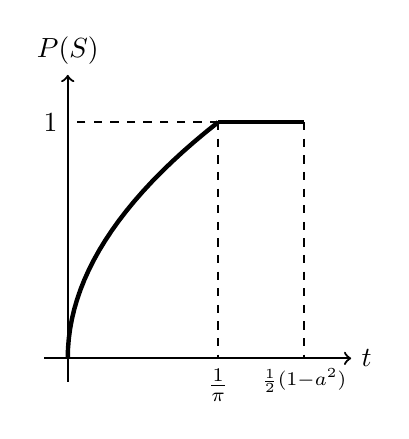
\begin{tikzpicture}[scale=3]
            \draw[->,thick] (-0.1,0) -- (1.2,0) node[anchor= west] {$t$};
            \draw[->,thick] (0,-0.1) -- (0,1.2) node[anchor=south] {$P(S)$};
            \draw[ultra thick,domain=0:1] plot(0.637*\x*\x,\x);
            \draw[ultra thick] (0.637,1) -- (1,1);
            \draw[thick,dashed] (0.637,1) -- (0.637,0) node[anchor=north] {$\frac{1}{\pi}$};
            \draw[thick,dashed] (1,1) -- (1,0) node[anchor=north] {$\scriptstyle \frac{1}{2}(1-a^2)$};
            \draw[thick,dashed] (0.637,1) -- (0,1) node[anchor=east] {$1$};
        \end{tikzpicture}
    \end{center}
    \item $\alpha \leq a \leq \beta$
    \begin{center}
        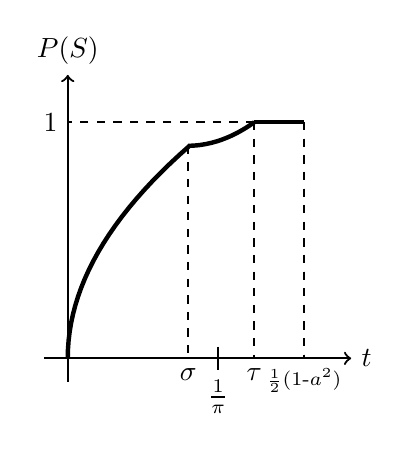
\begin{tikzpicture}[scale=3]
            \draw[->,thick] (-0.1,0) -- (1.2,0) node[anchor= west] {$t$};
            \draw[->,thick] (0,-0.1) -- (0,1.2) node[anchor=south] {$P(S)$};
            \draw[ultra thick,domain=0:0.9] plot(0.637*\x*\x,\x);
            \draw[ultra thick] (0.79,1) -- (1,1);
            \draw[thick,dashed] (0.51,0.9) -- (0.51,0) node[anchor=north] {$\sigma$};
            \draw[thick,dashed] (0.79,1) -- (0.79,0) node[anchor=north] {$\tau$};
            \draw[thick,dashed] (1,1) -- (1,0);
            \draw[thick,dashed] (0.79,1) -- (0,1) node[anchor=east] {$1$};
            \draw[ultra thick] (0.51,0.9) parabola (0.79,1);
            \draw[thick] (0.637,0.05) -- (0.637,-0.05) node[anchor=north] {$\frac{1}{\pi}$};
            \draw[thick,dashed] (1,1) -- (1,0) node[anchor=north] {$\scriptstyle \frac{1}{2}(1\text{-}a^2)$};
        \end{tikzpicture}
        \hspace{1em}
        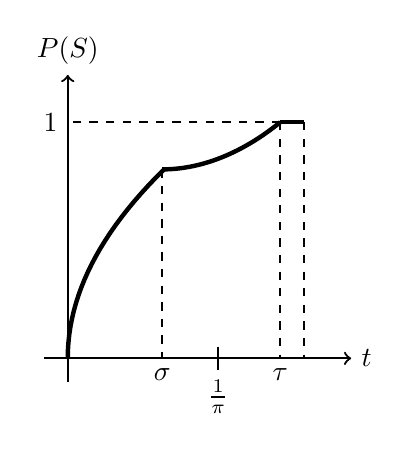
\begin{tikzpicture}[scale=3]
            \draw[->,thick] (-0.1,0) -- (1.2,0) node[anchor= west] {$t$};
            \draw[->,thick] (0,-0.1) -- (0,1.2) node[anchor=south] {$P(S)$};
            \draw[ultra thick,domain=0:0.8] plot(0.637*\x*\x,\x);
            \draw[ultra thick] (0.9,1) -- (1,1);
            \draw[thick,dashed] (0.4,0.8) -- (0.4,0) node[anchor=north] {$\sigma$};
            \draw[thick,dashed] (0.9,1) -- (0.9,0) node[anchor=north] {$\tau$};
            \draw[thick] (0.637,0.05) -- (0.637,-0.05) node[anchor=north] {$\frac{1}{\pi}$};
            \draw[thick,dashed] (1,1) -- (1,0);
            \draw[thick,dashed] (0.9,1) -- (0,1) node[anchor=east] {$1$};
            \draw[ultra thick] (0.4,0.8) parabola (0.9,1);
        \end{tikzpicture}
    \end{center}
    \item $\beta \leq a \leq \gamma$
    \begin{center}
        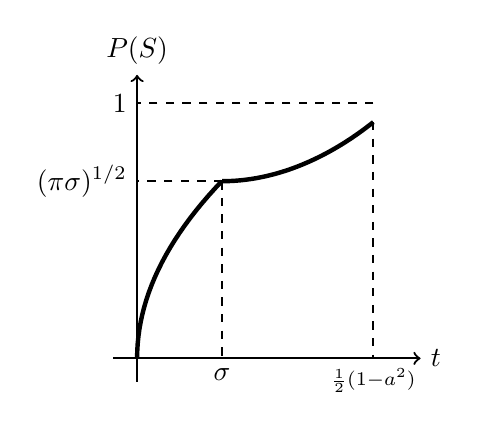
\begin{tikzpicture}[scale=3]
            \draw[->,thick] (-0.1,0) -- (1.2,0) node[anchor= west] {$t$};
            \draw[->,thick] (0,-0.1) -- (0,1.2) node[anchor=south] {$P(S)$};
            \draw[ultra thick,domain=0:0.75] plot(0.637*\x*\x,\x);
            \draw[thick,dashed] (0.36,0.75) -- (0.36,0) node[anchor=north] {$\sigma$};
            \draw[thick,dashed] (1,1) -- (1,0) node[anchor=north] {$\scriptstyle \frac{1}{2}(1-a^2)$};
            \draw[thick,dashed] (1,1.08) -- (0,1.08) node[anchor=east] {$1$};
            \draw[thick,dashed] (0.36,0.75) -- (0,0.75) node[anchor=east] {$(\pi \sigma)^{1/2}$};
            \draw[ultra thick] (0.36,0.75) parabola (1,1);
        \end{tikzpicture}
    \end{center}
    \item $\gamma \leq a \leq 1$
    \begin{center}
        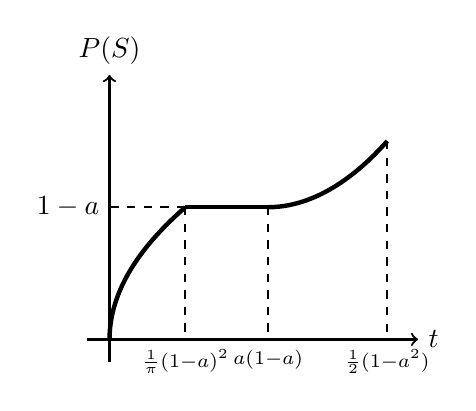
\begin{tikzpicture}[scale=2.8]
            \draw[->,thick] (-0.1,0) -- (1.4,0) node[anchor= west] {$t$};
            \draw[->,thick] (0,-0.1) -- (0,1.2) node[anchor=south] {$P(S)$};
            \draw[ultra thick,domain=0:0.6] plot(0.955*\x*\x,\x);
            \draw[ultra thick] (0.344,0.6) -- (0.72,0.6);
            \draw[thick,dashed] (0.344,0.6) -- (0.344,0) node[anchor=north] {$\scriptstyle\frac{1}{\pi}(1-a)^2$};
            \draw[thick,dashed] (0.72,0.6) -- (0,0.6) node[anchor=east] {$1-a$};
            \draw[thick,dashed] (0.72,0.6) -- (0.72,0) node[anchor=north] {$\scriptstyle a(1-a)$};
            \draw[ultra thick] (0.72,0.6) parabola (1.26,0.9);
            \draw[thick,dashed] (1.26,0.9) -- (1.26,0) node[anchor=north] {$\scriptstyle \frac{1}{2}(1-a^2)$};
        \end{tikzpicture}
        \hspace{0.5em}
        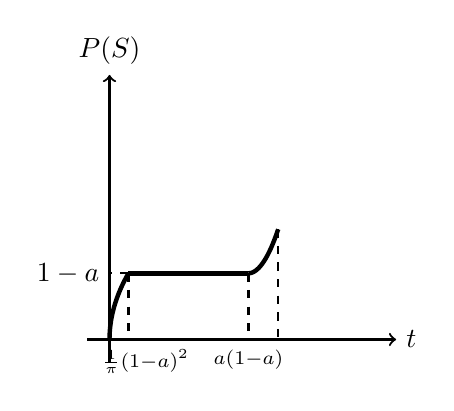
\begin{tikzpicture}[scale=2.8]
            \draw[->,thick] (-0.1,0) -- (1.3,0) node[anchor= west] {$t$};
            \draw[->,thick] (0,-0.1) -- (0,1.2) node[anchor=south] {$P(S)$};
            \draw[ultra thick,domain=0:0.3] plot(0.955*\x*\x,\x);
            \draw[ultra thick] (0.086,0.3) -- (0.63,0.3);
            \draw[thick,dashed] (0.086,0.3) -- (0.086,0) node[anchor=north] {$\scriptstyle\phantom{==}\frac{1}{\pi}(1-a)^2$};
            \draw[thick,dashed] (0.086,0.3) -- (0,0.3) node[anchor=east] {$1-a$};
            \draw[thick,dashed] (0.63,0.3) -- (0.63,0) node[anchor=north] {$\scriptstyle a(1-a)$};
            \draw[ultra thick] (0.63,0.3) parabola (0.765,0.5);
            \draw[thick,dashed] (0.765,0.5) -- (0.765,0);
        \end{tikzpicture}
    \end{center}
\end{itemize}










\bibliographystyle{plain}
\bibliography{biblio}

\end{document}
